\documentclass[12pt,a4paper,english,brazilian,oneside,chapter=TITLE,section=TITLE]{abntex2}

\usepackage{geometry}
\usepackage{graphicx}
\usepackage{tikz}
\usepackage{tikz-uml}
\usepackage{float}
\usepackage{algorithm}
\usepackage{algpseudocode}
\usepackage{siunitx}
\usepackage[alf]{abntex2cite}
\usepackage{plantuml}

\usepackage{indentfirst}

\usepackage[acronym]{glossaries}
\makeglossaries

\geometry{top=3cm, bottom=2cm, left=3cm, right=2cm}
\setlength{\parindent}{1.25cm}

\usetikzlibrary{positioning, arrows.meta, fit, calc}
\tikzset{
  initial/.style={circle, fill},
  decision/.style={diamond, black, draw},
  action/.style={rectangle, draw, rounded corners},
  arrow/.style={draw, -{Latex[length=3mm]}, thick}
}

\titulo{Um Hipervisor Tipo-1 Leve de Tempo Real para Sistemas Embarcados RISC-V: Projeto e Implementação em C++}
\autor{Ilton Pfleger Júnior}
\local{Florianópolis}
\data{2027}
\orientador{Antônio Augusto Fröhlich}
\instituicao{Universidade Federal de Santa Catarina}
\tipotrabalho{Trabalho de Conclusão de Curso}
\preambulo{}

\begin{document}

\imprimircapa
\imprimirfolhaderosto

\pdfbookmark[0]{\listfigurename}{lof}
\listoffigures*
\cleardoublepage

\pdfbookmark[0]{\contentsname}{toc}
\tableofcontents*
\cleardoublepage

\newglossaryentry{riscv}{
	name={RISC-V},
	plural={RISC-V},
	description={Conjunto de instruções de máquina livre para ser usado para qualquer finalidade, permitindo a qualquer pessoa ou empresa projetar e vender chips RISC-V sem precisar pagar royalties}
}

\newglossaryentry{cpu}{
	name={CPU},
	plural={CPUs},
	description={Parte central do computador, responsável por interpretar e executar instruções, realizar cálculos e processar dados}
}

\newglossaryentry{sistema-embarcado}{
	name={Sistema Embarcado},
	text={sistema embarcado},
	plural={sistemas embarcados},
	description={Um computador pequeno feito para executar uma tarefa específica dentro de outro equipamento}
}

\newglossaryentry{hardware} {
	name={Hardware},
    text={hardware},
	plural={hardwares},
	description={Parte física e tangível de um computador}
}

\newglossaryentry{mediador-de-hardware} {
	name={Mediador de Hardware},
    text={mediador de hardware},
    plural={mediadores de hardware},
	description={Um componente de software que encapsula, gerencia e abstrai dispositivos físicos}
}


\newacronym{api}{API}{Interface de Programação de Aplicações}

\newacronym[
plural={SOs},
longplural={Sistemas Operacionais}
]{so}{SO}{Sistema Operacional}

\newacronym[
plural={RTOSs},
longplural={Sistemas Operacionais de Tempo Real}
]{rtos}{RTOS}{Sistema Operacional de Tempo Real}

\newacronym[
plural={GPOSs},
longplural={Sistemas Operacionais de Propósito Geral}
]{gpos}{GPOS}{Sistema Operacional de Propósito Geral}

\newacronym[
plural={GPUs},
longplural={Unidades de Processamento Gráfico}
]{gpu}{GPU}{Unidade de Processamento Gráfico}

\newacronym[
plural={MMUs},
longplural={Unidades de Gerenciamento de Memória}
]{mmu}{MMU}{Unidade de Gerenciamento de Memória}

\newacronym[
plural={VMMs},
longplural={Monitores de Máquinas Virtuais}
]{vmm}{VMM}{Monitor de Máquina Virtual}


\newacronym[
plural={ISAs},
longplural={Instruction Set Architectures}
]{isa}{ISA}{Instruction Set Architecture}

\newacronym[
plural={RISCs},
longplural={Reduced Instruction Set Computers}
]{risc}{RISC}{Reduced Instruction Set Computer}

\newacronym[
plural={CSRs},
longplural={Control and Status Registers}
]{csr}{CSR}{Control and Status Register}


\textual

\chapter{Introdução}

Sistemas embarcados estão presentes em uma ampla gama de aplicações, que vão desde dispositivos médicos e sistemas de automação industrial
até plataformas automotivas e missões espaciais. Diferentemente da computação de propósito geral, esses sistemas operam sob rigorosos requisitos
de tempo real, nos quais a corretude do comportamento não depende apenas da precisão lógica dos resultados produzidos, mas também do momento
exato em que esses resultados são disponibilizados. Em muitos casos, atrasos mínimos ou falhas temporais podem comprometer a segurança, a
confiabilidade e até mesmo a integridade física de pessoas e equipamentos.

Tradicionalmente, a garantia desse determinismo esteve associada ao uso de plataformas dedicadas, nas quais \glspl{rtos} são empregados para assegurar
previsibilidade temporal, isolamento entre tarefas e cumprimento de restrições rígidas de escalonamento. Entretanto, a evolução do software contemporâneo
deslocou grande parte dos ecossistemas de desenvolvimento — bibliotecas, frameworks, ferramentas e serviços — para ambientes baseados em \glspl{gpos} - 
especialmente Linux. Embora esses sistemas ofereçam grande riqueza funcional e amplo suporte da comunidade, sua adoção em contextos críticos embarcados demanda
esforços adicionais de adaptação, validação e integração.

Como resultado, cresce a necessidade de consolidar, em uma mesma plataforma computacional, cargas de trabalho com requisitos distintos e frequentemente
conflitantes: de um lado, aplicações críticas, sensíveis a prazos temporais e dependentes de comportamento determinístico; de outro, aplicações complexas,
orientadas a funcionalidades avançadas e dependentes de ambientes generalistas.

Nesse cenário, técnicas de virtualização surgem como uma alternativa promissora, pois permitem a coexistência de múltiplos ambientes de execução sobre o
mesmo hardware. Dessa forma, torna-se possível executar aplicações críticas e não críticas de maneira controlada, reduzindo custos de integração e
aumentando o aproveitamento da plataforma.

Paralelamente, a arquitetura aberta RISC-V vem ganhando relevância  devido à sua flexibilidade, modularidade e independência
tecnológica. Seu conjunto de instruções extensível, aliado à ausência de barreiras proprietárias, favorece tanto a pesquisa acadêmica quanto o desenvolvimento
industrial, especialmente em soluções customizadas e de baixo custo.

Por isso, este trabalho propõe o projeto e a implementação, utilizando a linguagem C++ orientada a objetos de baixo overhead, de uma infraestrutura de virtualização para sistemas
baseados em RISC-V. O foco principal reside na previsibilidade temporal, no isolamento rígido entre cargas de trabalho e no baixo custo de execução. Busca-se, assim, contribuir para
a viabilização de plataformas embarcadas capazes de integrar aplicações heterogêneas sem comprometer requisitos críticos de desempenho e confiabilidade.

\section{Objetivos}

\subsection{Objetivos Gerais}

Projetar, implementar e validar uma infraestrutura de virtualização de baixo overhead para sistemas embarcados baseados na arquitetura RISC-V, utilizando a linguagem C++,
com foco no isolamento de cargas de trabalho, no particionamento estático de recursos e na previsibilidade temporal necessária à execução de aplicações de tempo real.

\subsection{Objetivos Específicos}

\begin{enumerate}
\item Definir a arquitetura de software do hipervisor, estabelecendo os mecanismos necessários para o gerenciamento e isolamento das máquinas virtuais.
\item Implementar o núcleo de virtualização responsável pela criação, inicialização, gerenciamento e execução das máquinas virtuais em plataformas RISC-V.
\item Desenvolver mecanismos de virtualização de interrupções e exceções, assegurando o tratamento correto e eficiente dos eventos entre hardware, hipervisor e sistemas convidados.
\item Implementar mecanismos de particionamento estático e isolamento de recursos computacionais, incluindo processadores, memória e dispositivos de entrada e saída.
\item Garantir a execução isolada de aplicações com diferentes requisitos operacionais, possibilitando a coexistência de cargas de trabalho críticas e não críticas em uma mesma plataforma computacional.
\item Validar funcionalmente a infraestrutura desenvolvida por meio da execução de sistemas convidados representativos.
\item Avaliar o impacto da virtualização sobre métricas relacionadas ao desempenho e à previsibilidade temporal, incluindo latência, tempo de resposta e sobrecarga de execução.
\end{enumerate}


\chapter{Fundamentação Teórica}

\section{Sistemas Embarcados}

Sistemas embarcados são soluções computacionais projetadas para executar funções dedicadas no interior de equipamentos maiores. Amplamente utilizados em setores como automação industrial,
indústria automotiva, medicina, telecomunicações e \gls{iot}, esses sistemas destacam-se pela forte integração entre hardware e software. Como operam frequentemente sob restrições severas de
processamento, memória, armazenamento e consumo de energia, exigem um desenvolvimento altamente otimizado para entregar máxima eficiência com baixo custo computacional.

\section{Sistemas Operacionais}

Um sistema operacional é um software responsável por gerenciar os recursos de hardware de um sistema computacional e fornecer serviços para a execução de aplicações.
Atuando como uma camada de abstração entre o hardware e os programas, o sistema operacional simplifica o desenvolvimento de software ao oferecer mecanismos padronizados
para acessar o processador, memória, dispositivos de entrada e saída, dispositivos armazenamento de dados, etc.

A evolução dos sistemas operacionais permitiu o surgimento de plataformas cada vez mais complexas, capazes de executar múltiplas aplicações simultaneamente e
fornecer diversos serviços ao usuário. Entretanto, dependendo dos requisitos da aplicação, características como previsibilidade temporal, confiabilidade e isolamento podem
se tornar tão importantes quanto o desempenho, motivando o desenvolvimento de sistemas operacionais especializados.

\section{Sistemas De Tempo Real}

Sistemas que operam sob restrições de tempo real são sistemas nos quais a reatividade temporal é extremamente importante para a corretude ou até mesmo para a
segurança do ambiente de execução. Nesses sistemas, não é suficiente que uma operação produza um resultado correto ou que seja extremamente rápida, sendo também necessário que esse resultado
seja produzido dentro de um intervalo de tempo determinado \cite{stankovic1988misconceptions}. 

Para atender a esses requisitos, são empregados \glspl{rtos}, projetados para fornecer mecanismos de gerenciamento de tarefas e recursos que favoreçam a previsibilidade e o cumprimento de
restrições temporais. Diferentemente de \glspl{gpos}, nos quais o objetivo principal geralmente está relacionado ao aumento do desempenho médio, da utilização dos
recursos ou da responsividade percebida pelo usuário, um \gls{rtos} prioriza a capacidade de determinar e controlar os tempos envolvidos na execução das tarefas.

Os conceitos centrais associados aos \glspl{rtos} são o \textit{deadline} e o determinismo. O \textit{deadline} - ou prazo limite - refere-se ao instante máximo em que a execução de uma
determinada tarefa deve ser concluída, cabendo ao \gls{rtos} gerenciar os recursos para assegurar o cumprimento desta restrição. Por sua vez, o determinismo — frequentemente associado
à previsibilidade do sistema — garante que o comportamento temporal do software seja conhecido e limitado, com a determinação do tempo de execução no pior caso ou \gls{wcet}.

O elemento central do núcleo de um \gls{rtos} que viabiliza essa previsibilidade é o algoritmo de escalonamento de tarefas  - adaptado para tempo real.
Entre os algoritmos mais consolidados na literatura, destacam-se o \gls{edf}, utilizado em cenários com prioridades dinâmicas — nos quais o conjunto de tarefas ou seus prazos podem
variar em tempo de execução —, e o \gls{rm}, voltado a cenários estáticos, onde as tarefas e seus períodos de ativação são totalmente conhecidos em fase de projeto.

\subsection{Classificação De Sistemas De Tempo Real}

Tais sistemas são classificados de acordo com as consequências do não cumprimento dos requisitos temporais definidos em sua elaboração.
Sistemas nos quais a perda de um prazo pode causar danos catastróficos, como a perda de vidas humanas ou a destruição de equipamentos de alto valor, são classificados como Hard Real-Time.
Por outro lado, sistemas nos quais o atraso temporal não é desejável, mas também não é fatal ou crítico — como o atraso na entrega de quadros em serviços de vídeo —, são chamados de Soft Real-Time.

\subsection{Outros Aspectos De Previsibilidade Temporal}

\begin{itemize}
    \item \textbf{Latência:} intervalo de tempo entre a ocorrência de um evento e o início da ação correspondente do sistema.

    \item \textbf{\textit{Jitter}:} variação temporal observada na latência ou no instante de ocorrência de eventos em relação ao comportamento esperado.

    \item \textbf{\textit{Overhead}:} custo computacional adicional introduzido por algum mecanismo.
\end{itemize}




\section{Virtualização}

Virtualização é uma técnica computacional que permite a execução simultânea e isolada de múltiplos \glspl{so} — denominados sistemas convidados — em um mesmo hardware físico.
Enquanto um \gls{so} convencional atua como uma interface entre o usuário e a máquina, abstraindo a complexidade da arquitetura subjacente, existem sistemas projetados
para estender essa abstração a outros \glspl{so}. Esses sistemas são denominados hipervisores, e o mecanismo que viabiliza esse processo é chamado de virtualização.

De modo geral, existem dois principais tipos de virtualização: a virtualização completa e a paravirtualização.

Na virtualização completa, também conhecida como \textit{full virtualization}, o \gls{so} convidado executa sem ter conhecimento explícito de que está em um ambiente virtualizado.
Nesse cenário, operações privilegiadas são interceptadas pelo hipervisor por meio de exceções e tratadas por mecanismos como \textit{trap-and-emulate}.
Entretanto, esse processo pode comprometer o desempenho do sistema, devido ao custo associado às operações de salvamento e restauração de contexto realizadas a cada exceção gerada.

Em contraste, a paravirtualização adota uma abordagem cooperativa entre o \gls{so} convidado e o seu hipervisor.
Nesse modelo, o sistema convidado é modificado para reconhecer a presença do ambiente virtualizado e, em vez de executar diretamente instruções privilegiadas,
realiza chamadas explícitas ao hipervisor, conhecidas como \textit{hypercalls}. Essa estratégia reduz a necessidade de exceções, diminuindo o custo associado ao processo de virtualização.

\section{Interceptação e Emulação}

Do inglês \textit{trap-and-emulate}, interceptação e emulação trata-se de um método utilizado para viabilizar a virtualização em sistemas nos quais o suporte de
hardware não é completamente implementado. Nesse modelo, quando a aplicação executada em ambiente virtualizado tenta realizar uma operação que depende de recursos privilegiados,
essa operação é interceptada e tratada como uma exceção. O controle é então transferido para um nível mais privilégiado, geralmente o hipervisor, que fica responsável por
emular em software o comportamento esperado da instrução ou operação originalmente solicitada.

\begin{figure}[H]
\centering
\includegraphics[width=0.8\textwidth]{images/TrapAndEmulate.pdf}
\caption{Fluxograma de Interceptação de Instruções Privilegiadas}\label{fig:trap-and-emulate}
\end{figure}



\section{\textit{VirtIO}}

\textit{VirtIO} \cite{Rusty-Russell-VirtIO} é um padrão para drivers de dispositivos paravirtualizados, projetado para unificar e otimizar a interface de comunicação entre os
sistemas convidados e o hipervisor. Em vez de emular hardwares legados complexos e específicos, o hipervisor expõe uma série de dispositivos virtuais padronizados, permitindo que
o \gls{so} convidado acesse recursos de rede, armazenamento e console de maneira eficiente e com baixa sobrecarga.

Para viabilizar essa comunicação, o modelo utiliza as chamadas \textit{Virtqueues} — filas circulares compartilhadas responsáveis pelo envio e recebimento das requisições.
Dependendo das operações suportadas, cada dispositivo virtual pode alocar uma ou mais dessas filas. Internamente, uma \textit{Virtqueue} divide-se em três componentes principais:
uma tabela de descritores (\textit{Descriptor Table}), um anel de índices disponíveis (\textit{Available Ring}) e um anel de índices já utilizados (\textit{Used Ring}).

Na prática, o ciclo de vida de uma operação de \gls{io} ocorre em duas etapas complementares. Inicialmente, quando o sistema convidado deseja realizar uma operação, o dispositivo \textit{VirtIO}
escreve os dados na memória compartilhada, insere o descritor correspondente no \textit{Available Ring} e notifica o hipervisor sobre a nova pendência. 

Em resposta, o hipervisor consome os descritores desse anel, processa a operação solicitada e registra o resultado no \textit{Used Ring}. Por fim, uma interrupção
é enviada ao sistema convidado para sinalizar a conclusão da tarefa. Graças a esse design, múltiplas requisições podem ser tratadas de maneira assíncrona e em lote, o que minimiza
as trocas de contexto e reduz expressivamente o custo inerente à virtualização.

Desse modo, o \textit{VirtIO} consolida-se como uma solução fundamental para a infraestrutura de virtualização moderna, pois alcança um equilíbrio entre a flexibilidade de uma interface padronizada e o
desempenho da paravirtualização.

\section{Hipervisors}

Um hipervisor, também conhecido como \gls{vmm}, é uma plataforma que cria e executa máquinas virtuais via virtualização.
Segundo \citeonline{PopekGeraldGoldberg} um \gls{vmm} possuí três características essenciais: primeiro, devem fornecer um ambiente idêntico à máquina original
para programas; segundo, os programas executados nesse ambiente, na pior das hipóteses, devem apresentar no máximo pequenas reduções
de velocidade que urgem da camada de virtualização; e por último, os \glspl{vmm} devem deter o contole total sobre os recursos do sistema.

Na visão de \cite{Goldberg}, fundamentalmente, existem dois tipos de hipervisores: 1 e 2.

\subsection{Tipo 1 - Bare Metal}

Hipervisores de tipo 1, também conhecidos como bare metal, são aqueles que executam diretamente sobre o hardware físico, sem a necessidade de um
sistema operacional hospedeiro intermediário.
Por operar diretamente sobre o hardware, esse tipo de hipervisor geralmente apresenta melhor desempenho e menor sobrecarga.

\begin{figure}[H]
    \centering
    \begin{tikzpicture}[
        pequeno/.style={
            draw,
            thick,
            fill=blue!5,
            minimum width=4cm,
            minimum height=1.2cm,
            outer sep=0pt
        }
    ]
        \node[pequeno] (apps-so1-1) {Aplicação 1};
        \node[pequeno, right=0.2cm of apps-so1-1] (apps-so1-2) {Aplicação 2};
        \node[pequeno, right=0.2cm of apps-so1-2] (apps-so2-1) {Aplicação 1};

        \node[fit=(apps-so1-1)(apps-so1-2), inner sep=0pt] (apps-so1) {};
        \node[fit=(apps-so2-1), inner sep=0pt] (apps-so2) {};

        \node[
            draw,
            thick,
            fill=blue!10,
            minimum width=8.2cm,
            minimum height=1.5cm,
            below=0.2cm of apps-so1
		] (SO1) {\Gls{so} 1};

		\node[
            draw,
            thick,
            fill=blue!10,
            minimum width=4cm,
            minimum height=1.5cm,
            below=0.2cm of apps-so2
		] (SO2) {\Gls{so} 2};

		\node[fit=(SO2)(SO1), inner sep=0pt] (SOs) {};

		\node[
            draw,
            thick,
            fill=blue!15,
            minimum width=12.4cm,
            minimum height=1.5cm,
            below=0.2cm of SOs
		] (HOS) {Hipervisor};

		\node[
            draw,
            thick,
            fill=blue!20,
            minimum width=12.4cm,
            minimum height=1.5cm,
            below=0.2cm of HOS
		] () {Hardware};

    \end{tikzpicture}
    \caption{Hipervisor Tipo 1.}
    \label{fig:hypervisor-type-1}
\end{figure}

\subsection{Tipo 2}

Diferentemente da solução bare metal, um hipervisor do tipo 2 é executado como um processo dentro de um \gls{so} hospedeiro.
Porém, apesar de garantir os mesmos recursos do tipo 1, sua arquitetura impõe uma camada intermediária a mais de software, o que restringe a
eficiência no acesso aos componentes físicos, gerando uma latência adicional e um menor desempenho.

\begin{figure}[H]
    \centering
    \begin{tikzpicture}[
        pequeno/.style={
            draw,
            thick,
            fill=blue!5,
            minimum width=4cm,
            minimum height=1.2cm,
            outer sep=0pt
        }
    ]
        \node[pequeno] (apps-so1-1) {Aplicação 1};
        \node[pequeno, right=0.2cm of apps-so1-1] (apps-so1-2) {Aplicação 2};
        \node[pequeno, right=0.2cm of apps-so1-2] (apps-so2-1) {Aplicação 1};

        \node[fit=(apps-so1-1)(apps-so1-2), inner sep=0pt] (apps-so1) {};
        \node[fit=(apps-so2-1), inner sep=0pt] (apps-so2) {};

        \node[
            draw,
            thick,
            fill=blue!10,
            minimum width=8.2cm,
            minimum height=1.5cm,
            below=0.2cm of apps-so1
		] (SO1) {\Gls{so} 1};

		\node[
            draw,
            thick,
            fill=blue!10,
            minimum width=4cm,
            minimum height=1.5cm,
            below=0.2cm of apps-so2
		] (SO2) {\Gls{so} 2};

		\node[fit=(SO2)(SO1), inner sep=0pt] (SOs) {};

		\node[
            draw,
            thick,
            fill=blue!15,
            minimum width=12.4cm,
            minimum height=1.5cm,
            below=0.2cm of SOs
		] (HOS) {Hipervisor};

		\node[
            draw,
            thick,
            fill=blue!20,
            minimum width=12.4cm,
            minimum height=1.5cm,
            below=0.2cm of HOS
		] (OS) {\Gls{so}};

		\node[
            draw,
            thick,
            fill=blue!25,
            minimum width=12.4cm,
            minimum height=1.5cm,
            below=0.2cm of OS
		] () {Hardware};

    \end{tikzpicture}
    \caption{Hipervisor Tipo 2.}
    \label{fig:hypervisor-type-2}
\end{figure}

\section{RISC-V}

A RISC-V é uma \gls{isa} baseada nos princípios \gls{risc}. Diferentemente de arquiteturas proprietárias,
a RISC-V possui uma especificação aberta e livre de \textit{royalties}, o que permite sua utilização tanto em contextos acadêmicos quanto em aplicações
comerciais.

Essa \gls{isa} define um conjunto básico de instruções, responsável pelas funcionalidades essenciais do processador. No entanto, sua
principal característica é a modularidade, permitindo que diferentes extensões sejam incorporadas conforme as necessidades da plataforma.
Dessa forma, é possível adaptar a arquitetura para cenários variados, desde sistemas embarcados com restrições de recursos até sistemas de
alto desempenho.

\subsection{Extensões Básicas}

\begin{description}

\item[I]
Adiciona suporte às instruções básicas de operações com números inteiros. Conforme descrito em~\cite{isa-riscv}, essa extensão deve estar
presente em qualquer implementação RISC-V, pois define as operações fundamentais de aritmética e manipulação de registradores.

\item[Zicsr]
Adiciona suporte às instruções de acesso e manipulação de \glspl{csr}.

\item[H]
Adiciona suporte ao modo H (Hipervisor).

\item[S]
Adiciona suporte ao modo S (Supervisor).

\item[M]
Adiciona suporte a operações de multiplicação e divisão de números inteiros.

\item[A]
Adiciona suporte a operações atômicas em memória.

\item[F]
Adiciona suporte a números em ponto flutuante de precisão simples (32 bits).

\item[D]
Adiciona suporte a números em ponto flutuante de precisão dupla (64 bits).

\item[C]
Adiciona suporte a instruções comprimidas de 16 bits.

\item[V]
Adiciona suporte a operações vetoriais para \gls{simd}.

\item[B]
Adiciona suporte à manipulação de bits em hardware, otimizando operações bit a bit.

\item[G]
Aglomerado geral de extensões (*General Purpose*) que inclui I, M, A, F, D e as extensões de controle Zicsr e Zifencei.

\end{description}

\subsection{Níveis de Privilégio}

Assim como a maior parte das arquiteturas modernas, a RISC-V utiliza um modelo hierárquico de privilégios para garantir a segurança e a estabilidade do sistema.
Esses níveis determinam quais operações e recursos de hardware podem ser acessados em cada contexto de execução. Os modos implementados em uma plataforma dependem
diretamente das extensões suportadas, estruturando-se tipicamente em três cenários principais:

\begin{itemize}

\item \textbf{Sem a extensão S:} Utiliza apenas o modo \textit{Machine} e o modo \textit{User}, indicado para sistemas embarcados mais simples e sem suporte a sistemas operacionais baseados em supervisor.
    \begin{figure}[H]
    \centering
    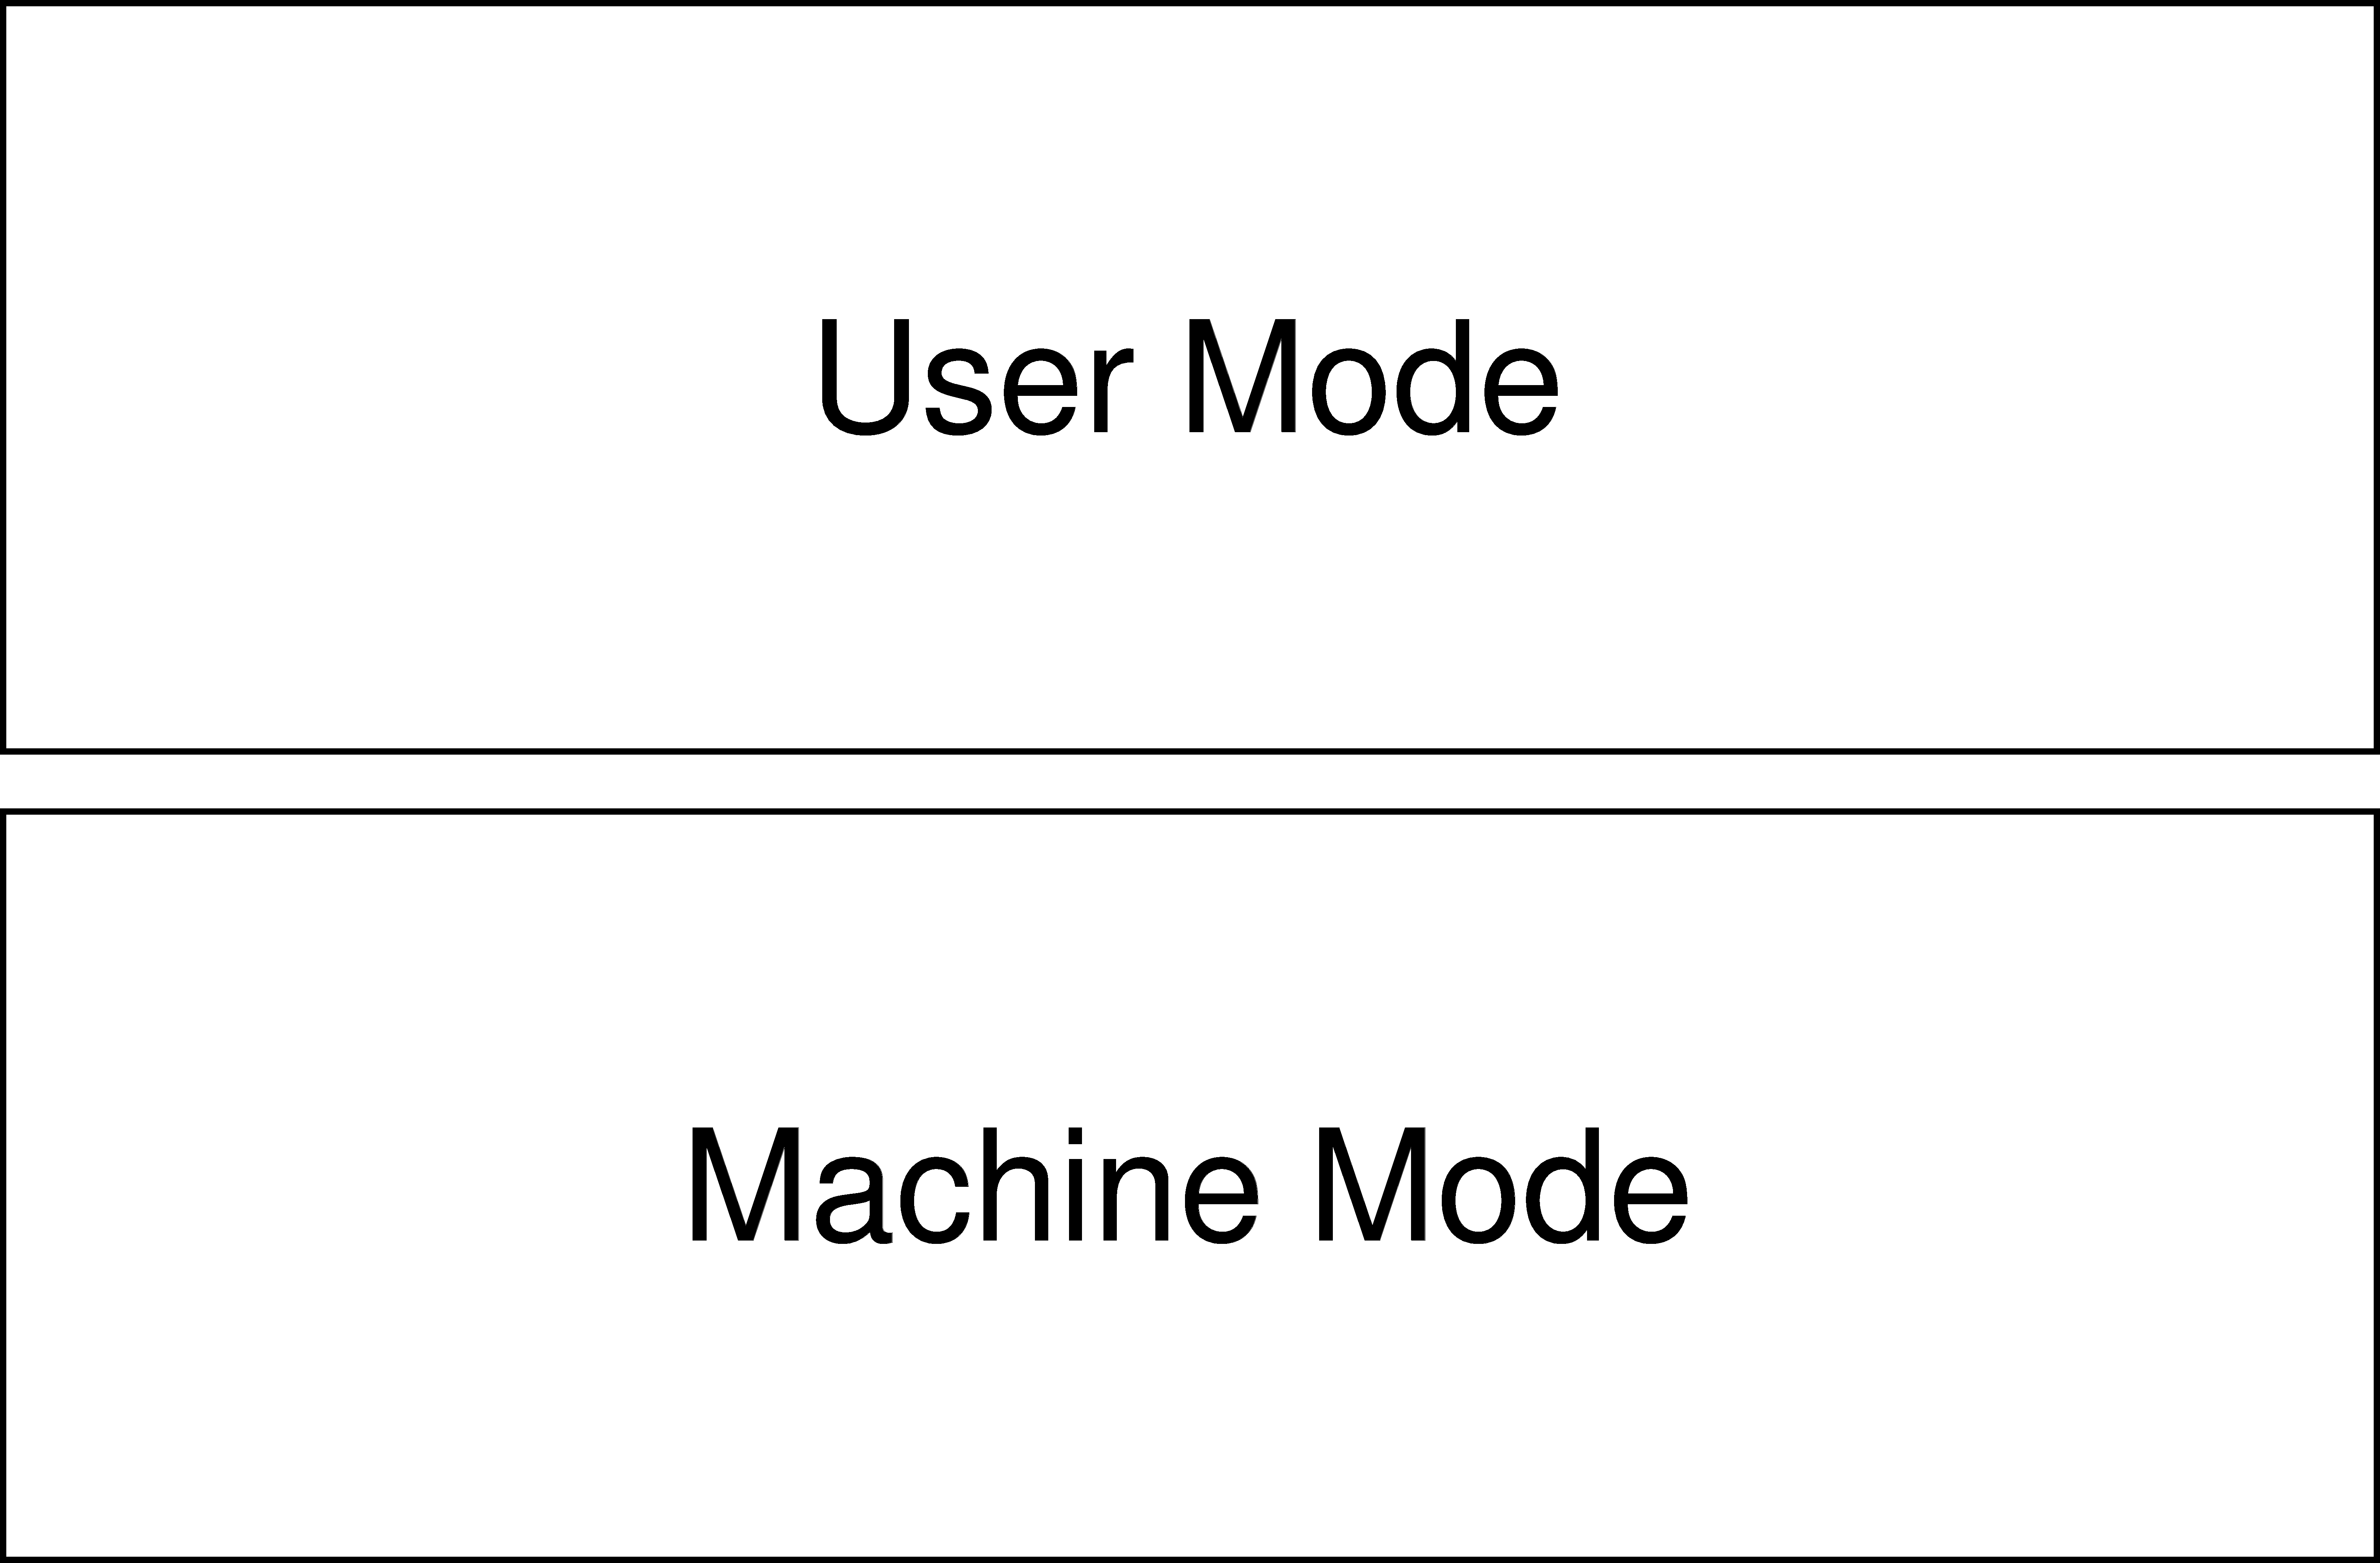
\includegraphics[width=0.3\textwidth]{images/MachineModeUserMode.pdf}
    \caption{Arquitetura de Privilégios RISC-V Sem Modo Supervisor}\label{fig:machine-mode-user-mode}
    \end{figure}

\item \textbf{Com a extensão S:} Adiciona o modo \textit{Supervisor}, permitindo a execução de sistemas operacionais completos que exigem isolamento entre o kernel e as aplicações de usuário.
    \begin{figure}[H]
    \centering
    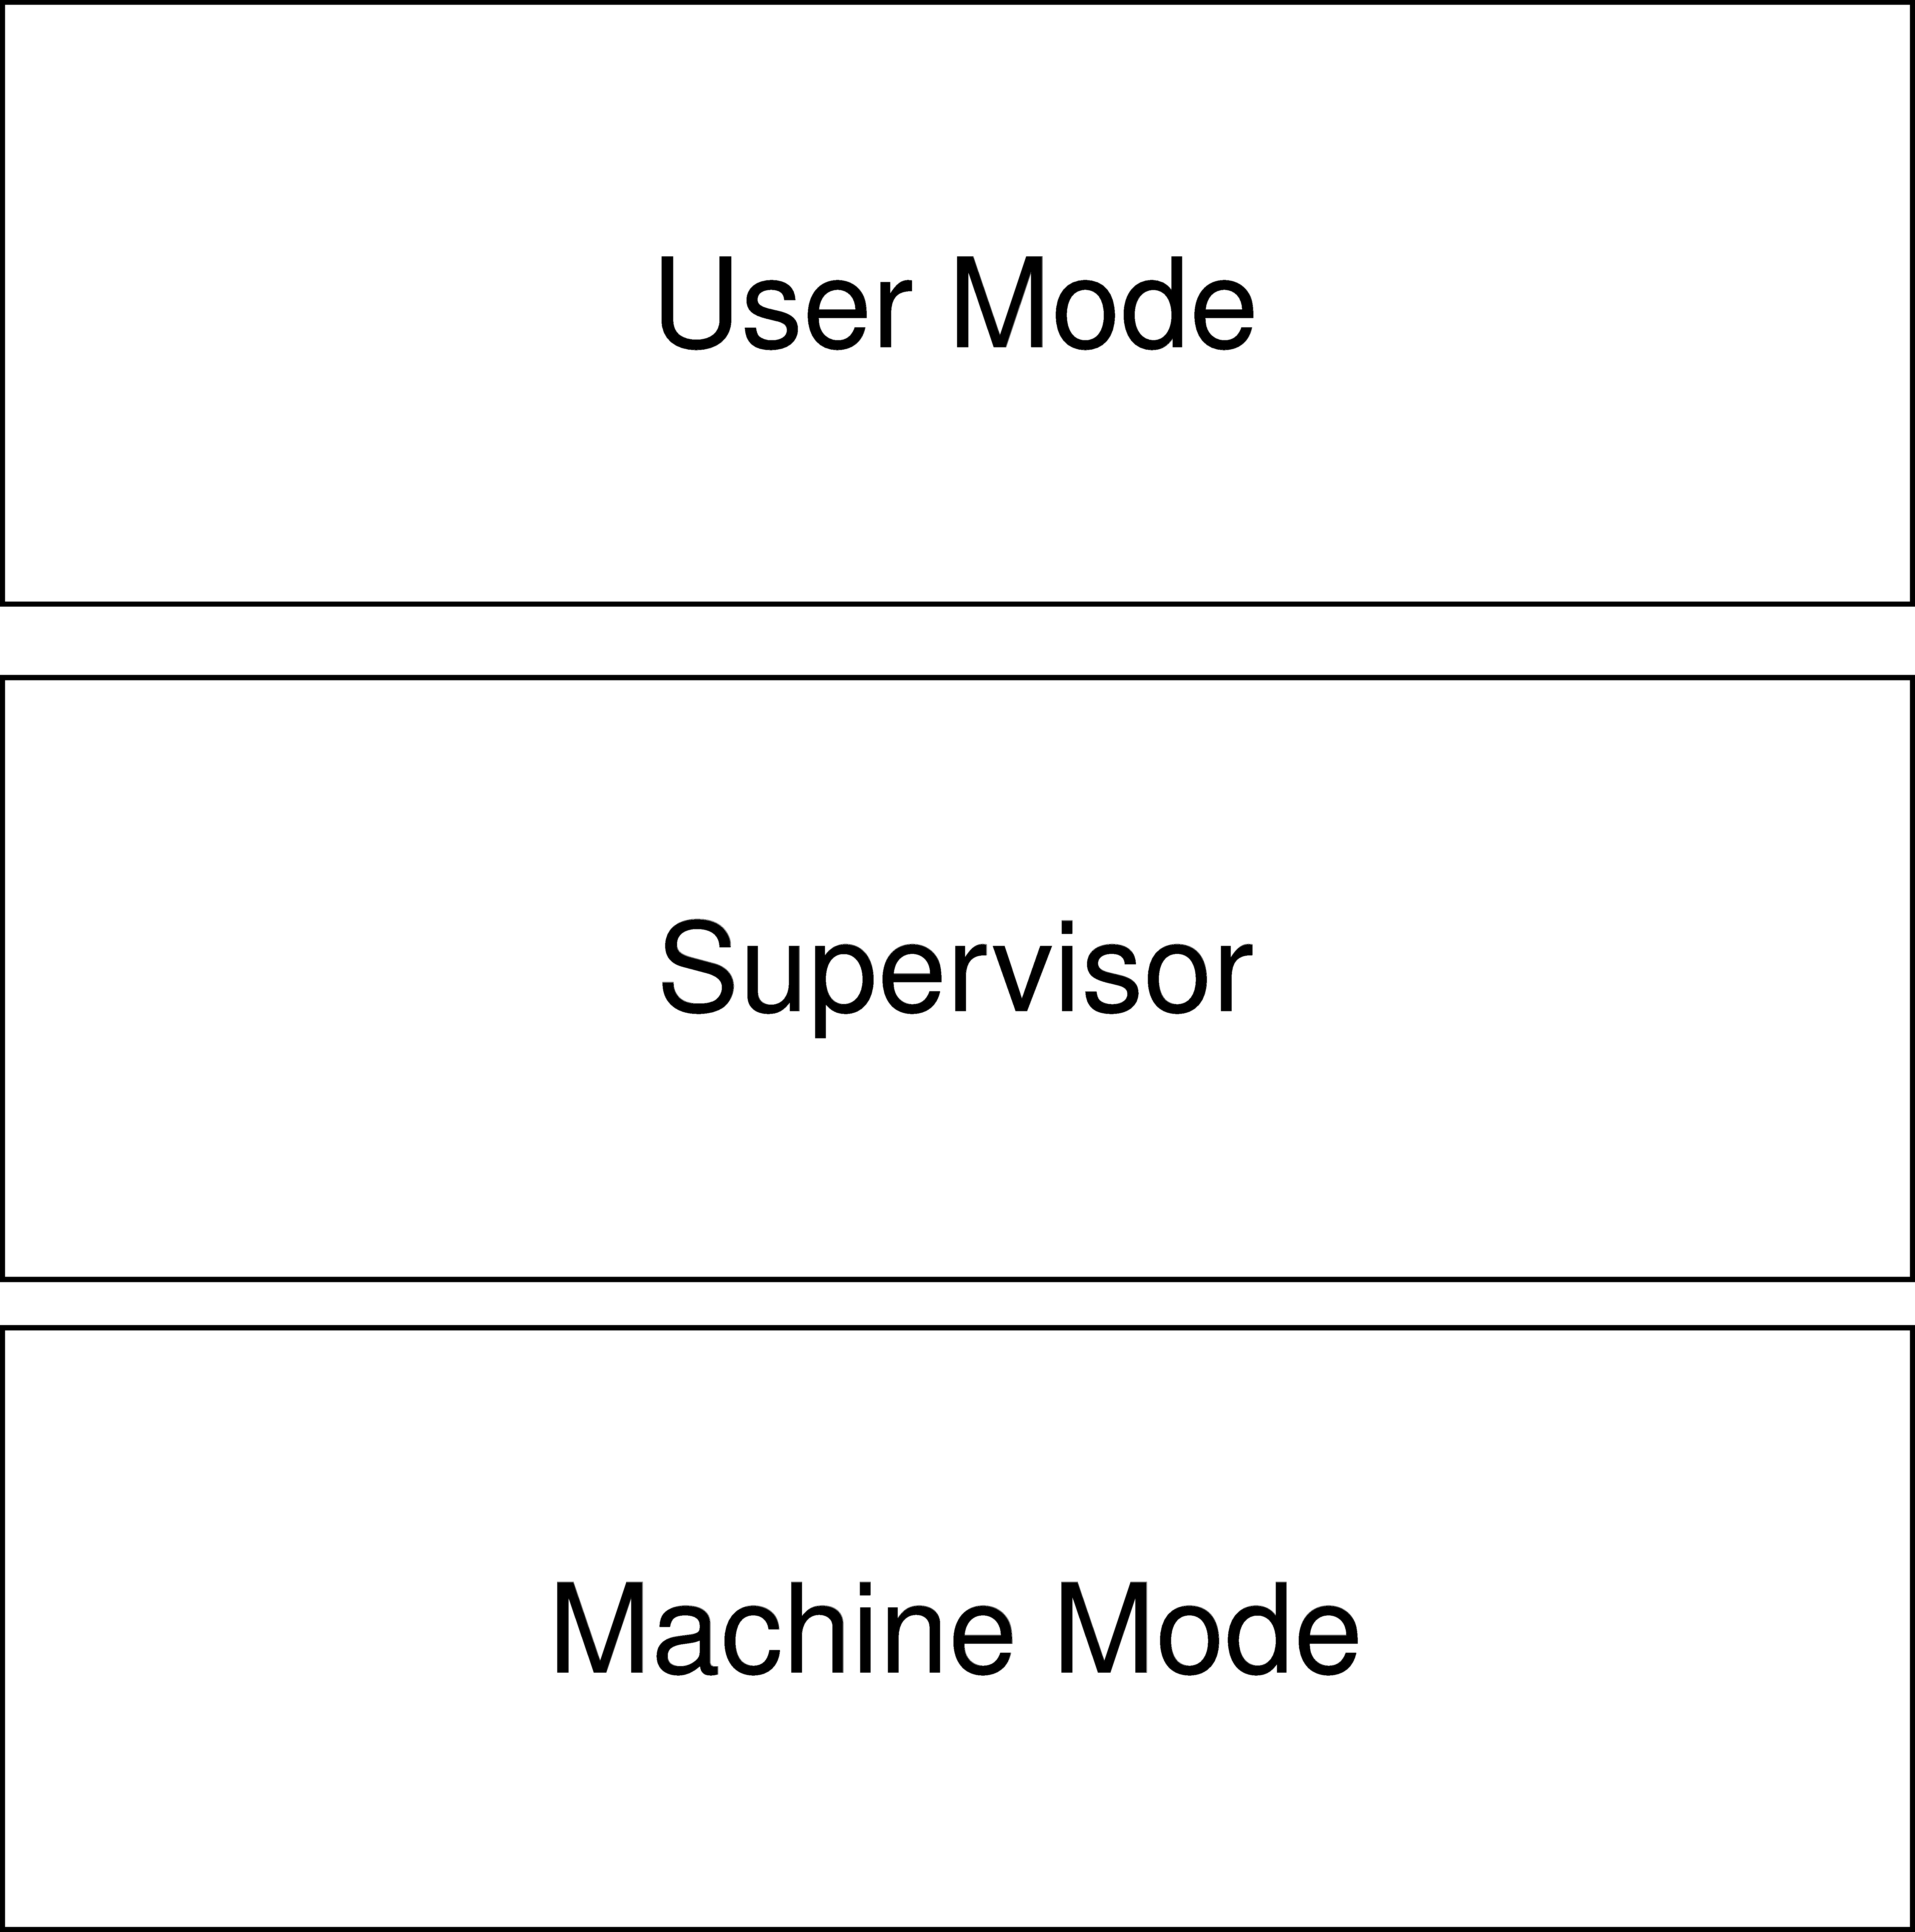
\includegraphics[width=0.3\textwidth]{images/SupervisorMode.pdf}
    \caption{Arquitetura de Privilégios RISC-V Com Modo Supervisor}\label{fig:machine-mode-user-mode-supervisor-mode}
    \end{figure}

\item \textbf{Com a extensão H:} Introduz o suporte aos modos \textit{Virtual User} e \textit{Virtual Supervisor}, estendendo os modos de privilégio para permitir a execução de hipervisores modernos.
    \begin{figure}[H]
    \centering
    \includegraphics[width=0.3\textwidth]{images/HypervisorMode.pdf}
    \caption{Arquitetura de Privilégios RISC-V Com Extensão H}\label{fig:riscv-hypervisor-mode}
    \end{figure}

\end{itemize}

\subsection{Registradores de Controle}

Os \glspl{csr} são registradores especiais utilizados para controlar e monitorar o funcionamento do processador. Eles armazenam informações essenciais relacionadas
ao estado da máquina, ao tratamento de exceções e interrupções, à configuração de privilégios e ao controle de funcionalidades específicas da arquitetura.

Esses registradores são organizados de forma segregada por nível de privilégio, sendo que cada nível dispõe do seu próprio conjunto de \glspl{csr}.
Esse isolamento é fundamental para a segurança e a integridade do sistema, pois garante uma política rígida de acessibilidade: um nível de privilégio só
pode acessar seus próprios registradores ou aqueles pertencentes a níveis menos privilegiados. Qualquer tentativa de acesso indevido a um \gls{csr} de um nível mais privilegiado 
resulta em uma exceção de instrução ilegal, impedindo que código menos privilegiado interfira diretamente nas camadas críticas do sistema.

Os principais \glspl{csr} são:

\begin{itemize}
    \item \texttt{mhartid}: mantém o identificador único de cada núcleo da CPU;\@
    \item \texttt{mstatus} e \texttt{mstatush}: mantêm os principais bits de configuração relacionados à arquitetura;
    \item \texttt{mtvec}: armazena o endereço base do vetor de manipuladores de exceções e interrupções no modo \textit{Machine};
    \item \texttt{mepc}: guarda o endereço da instrução que causou a exceção ou interrupção no modo \textit{Machine};
	\item \texttt{mcause}: armazena a causa de uma instrução ou exceção no modo \textit{Machine};
    \item \texttt{mtval}: armazena dados adicionais de uma exceção no modo \textit{Machine};
    \item \texttt{mscratch}: registrador temporário de rascunho usado para salvar ponteiros de contexto durante manipuladores no modo \textit{Machine};
    \item \texttt{mideleg} e \texttt{medeleg}: configuram a delegação de interrupções e exceções do modo \textit{Machine} para modos de menor privilégio;
    \item \texttt{mip}: mantém as interrupções atualmente pendentes;
    \item \texttt{mie}: mantém as interrupções atualmente habilitadas;
    \item \texttt{sstatus}: versão restrita e visível do registrador de status para o modo \textit{Supervisor};
    \item \texttt{stvec}: armazena o endereço base do manipulador de \textit{traps} no modo \textit{Supervisor};
    \item \texttt{sepc}: guarda o endereço da instrução que causou a exceção ou interrupção no modo \textit{Supervisor};
    \item \texttt{scause}: armazena a causa da interrupção ou exceção no modo \textit{Supervisor};
    \item \texttt{stval}: guarda informações adicionais relativas à exceção ocorrida no modo \textit{Supervisor};
    \item \texttt{sscratch}: registrador de rascunho temporário do modo \textit{Supervisor};
    \item \texttt{sip}: correspondente do modo \textit{Supervisor} ao \texttt{mip};
    \item \texttt{sie}: correspondente do modo \textit{Supervisor} ao \texttt{mie};
    \item \texttt{satp}: controla a tradução de endereços virtuais e a paginação da memória no modo \textit{Supervisor}.
\end{itemize}

\subsection{\gls{clint}}

O \gls{clint} é o mecanismo responsável por gerenciar interrupções locais — especificamente as de software e de temporização — em plataformas RISC-V.

Para a gestão de tempo, o \gls{clint} possui dois registradores centrais: \texttt{mtime} e \texttt{mtimecmp}. O \texttt{mtime} funciona como a referência temporal principal da arquitetura,
mantendo o \gls{so} ciente da passagem do tempo. O \texttt{mtimecmp}, por sua vez, determina o momento em que uma interrupção de temporização deve ser disparada:
quando o valor de \texttt{mtime} torna-se maior ou igual ao de \texttt{mtimecmp}, o \gls{clint} sinaliza o bit de interrupção temporal no registrador \gls{mip}.

Em relação às interrupções de software, o \gls{clint} disponibiliza um registrador \gls{msip} mapeado em memória para cada núcleo. Dessa forma, um núcleo pode disparar
uma interrupção de software em outro ativando o bit zero do registrador \gls{msip} pertencente ao núcleo de destino.

\subsection{\gls{plic}}

O funcionamento do \gls{plic} baseia-se na centralização e priorização de solicitações provenientes de periféricos externos. Quando uma interrupção atende aos requisitos
de habilitação e ao limiar de prioridade, o \gls{plic} notifica o núcleo ativando o bit correspondente de interrupção externa no registrador \gls{mip}, como \gls{meip} ou \gls{seip}.
A partir dessa notificação, para identificar e tratar a interrupção, o \gls{so} deve se comunicar ativamente com o \gls{plic}.

\subsection{Gerenciamento de Memória Virtual} 

A \gls{mmu} na arquitetura RISC-V é responsável por realizar a tradução de endereços virtuais em endereços físicos e por verificar as permissões de acesso à memória.
O mecanismo de tradução utilizado pelos sistemas operacionais é configurado por meio do registrador de controle \gls{satp}, disponível no modo \textit{Supervisor}.

Seu funcionamento baseia-se na paginação da memória, na qual os endereços virtuais são divididos em páginas, tipicamente com granularidade de 4,KiB. O \gls{so}
mantém tabelas de páginas que associam essas páginas virtuais a regiões da memória física e definem as permissões de acesso, como leitura, escrita e execução.
Dessa forma, quando um processo acessa um endereço virtual, a \gls{mmu} realiza a tradução correspondente e verifica se a operação solicitada é permitida.
Caso o endereço não esteja mapeado ou a operação viole as permissões estabelecidas, ocorre uma exceção de acesso à memória.

\subsection{Proteção de Memória Física}

Em sistemas que não possuem o modo supervisor --- ou como camada adicional de segurança ---, a arquitetura RISC-V emprega o mecanismo de \gls{pmp}.
Exclusivamente no modo \textit{Machine}, o firmware configura os registradores de \gls{pmp} para delimitar quais regiões da memória física podem ser acessadas pelos modos
\textit{User} e \textit{Supervisor}, assegurando o isolamento por hardware mesmo na ausência ou antes da inicialização de uma \gls{mmu}.

Para gerenciar essas regras, o mecanismo baseia-se em dois tipos de registradores: os registradores de configuração --- \textit{pmpcfg}, que definem as permissões de
acesso --- leitura, escrita e execução, o modo de pareamento de endereços e o bit de travamento para cada entrada; e os registradores de endereço --- \textit{pmpaddr},
que armazenam os endereços de referência ou parâmetros empregados pelo hardware para delimitar o tamanho e os limites das regiões protegidas.

O mecanismo de \gls{pmp} definido pela \gls{isa} da RISC-V possui três modos ativos de pareamento de endereços:

\begin{itemize}
    \item \textbf{\gls{tor}:} define uma faixa contínua de memória onde o registrador $\textit{pmpaddr}_i$ atua como o limite superior --- exclusivo --- e
        o registrador anterior $\textit{pmpaddr}_{i-1}$ atua como o limite inferior --- inclusivo. Para a primeira entrada ($i=0$), o limite inferior é considerado o
        endereço \textit{0$\times$0};
    \item \textbf{\gls{na4}:} mapeia um bloco fixo de exatamente 4 bytes apontado diretamente pelo registrador \textit{pmpaddr};
    \item \textbf{\gls{napot}:} define blocos com tamanhos que são potências de 2. O tamanho e o alinhamento da região são codificados nos bits menos significativos do próprio registrador \textit{pmpaddr}.
\end{itemize}

\subsection{Extensão H}

A extensão H introduz suporte nativo à virtualização em nível de hardware na arquitetura RISC-V. O principal objetivo dessa extensão é permitir a execução eficiente de um \gls{vmm}.
Para viabilizar esse isolamento e controle, a extensão H expande o modelo de privilégios da arquitetura, adicionando novos modos de execução:

\begin{itemize}
    \item \textbf{Virtual User:} modo no qual rodam as aplicações de usuário dentro do convidado.
    \item \textbf{Virtual Supervisor:} modo no qual o \gls{so} convidado é executado.
    \item \textbf{Hypervisor:} modo supervisor estendido, onde o hipervisor opera para gerenciar os recursos das \glspl{vm}.
\end{itemize}

\subsubsection{Tradução de Endereços em Dois Estágios}

Além dos novos modos de privilégio, a extensão H adiciona uma camada de tradução de memória para suportar a virtualização. Como múltiplos \glspl{so} convidados dependem da \gls{mmu} da plataforma
--- que normalmente seria controlada apenas pelo hipervisor ---, a arquitetura introduz os registradores \textit{vsatp} e \textit{hgatp} --- substitutos e complementos ao registrador padrão
\textit{satp} ---. Isso viabiliza uma tradução de endereços em dois estágios: o \textit{vsatp} mapeia os endereços virtuais do convidado para endereços físicos intermediários, enquanto o \textit{hgatp}
traduz esses endereços intermediários para a memória física real da máquina.

\begin{figure}[H]
\centering
\includegraphics[width=0.3\textwidth]{images/TwoStageMMU.pdf}
\caption{Tradução de Endereços em Dois Estágios da Extensão H}\label{fig:two-stage-mmu}
\end{figure}




\chapter{Materiais Utilizados}

Para a realização deste trabalho foi utilizada placa - \gls{sbc} - VisionFive 2. Considerando os objetivos propostos, as principais características de hardware
relevantes para este estudo são apresentadas a seguir:

\begin{itemize}
\item \gls{soc}: StarFive JH7110;
\item DRAM: 8 GB LPDDR4;
\item Interface Gigabit Ethernet: Synopsys DesignWare DWMAC 5.20;
\item PMIC: X-Powers AXP15060.
\end{itemize}

O \gls{soc} StarFive JH7110 opera com frequência de até 1,5 GHz e possui uma arquitetura heterogênea composta por seis núcleos de processamento, distribuídos da seguinte forma:

\begin{itemize}
\item 4 núcleos U74 de 64 bits, compatíveis com a arquitetura RISC-V RV64GC;
\item 1 núcleo S7 de 64 bits, compatível com a arquitetura RISC-V RV64IMAC;
\item 1 núcleo E24 de 32 bits, compatível com a arquitetura RISC-V RV32IMAFCB.
\end{itemize}

Cabe destacar que todos os experimentos realizados neste trabalho foram conduzidos utilizando essa placa. Além disso, foram considerados apenas os quatro núcleos U74,
uma vez que os núcleos S7 e E24 não oferecem suporte ao modo supervisor, requisito indispensável para a implementação dos mecanismos de virtualização aqui analisados.

\chapter{Metodologia}

\section{Virtualização Baseada \textit{Machine Mode}}

Originalmente, o \textit{Machine Mode} (M-mode) foi projetado para ser  o nível de privilégio mais elevado da arquitetura RISC-V, sendo
responsável pela execução do firmware base e pelo controle direto dos recursos de hardware.
Sua função primária consiste na inicialização da plataforma e na configuração dos subsistemas fundamentais antes da
transferência de controle para o \gls{so} hospedeiro.

Dada a natureza restritiva do acesso a determinados recursos de hardware — muitas vezes limitados exclusivamente ao M-mode —, a
arquitetura define camadas de abstração como a \gls{sbi}. Essa interface atua como uma ponte padronizada e segura, permitindo que
níveis de privilégio inferiores solicitem serviços privilegiados ao firmware residente no M-mode.

No contexto deste trabalho, o M-mode é utilizado de forma não convencional. Para isso, deixamos de usar o M-Mode como um simples
\gls{sbi} e passamos a usalo para dar suporte a implementação de um hipervisor completo.

Essa abordagem explora o fato de que o M-mode possui autoridade irrestrita sobre todos os demais níveis de privilégio, permitindo
interceptar, controlar e gerenciar a execução dos sistemas convidados. Para viabilizar esse controle, o hipervisor utiliza
os recursos exclusivos disponibilizados nesse modo, incluindo seu conjunto dedicado de \glspl{csr}, além de mecanismos próprios
para tratamento de interrupções e gerenciamento de temporização. Dessa forma, o M-mode fornece a soberania necessária
para reproduzir, por software, e as vezes até em hardware, funcionalidades que normalmente só seriam oferecidas por
hardwares especializados compatíveis com as extensões de virtualização.


\chapter{Implementação}

\section{Virtualização Baseada em Modo \textit{Machine}}

Originalmente, o modo \textit{Machine} da RISC-V foi projetado para ser o nível de privilégio mais elevado da arquitetura, sendo responsável pela execução de firmwares
e pelo controle direto dos recursos de hardware. Sua função primária consiste na inicialização da plataforma e na configuração dos subsistemas fundamentais antes da transferência
de controle para o \gls{so} hospedeiro.

Dada a natureza restritiva do acesso a determinados recursos de hardware — muitas vezes limitados exclusivamente a esse modo —, a arquitetura define camadas de
abstração como a \gls{sbi}. Essa interface atua como uma ponte padronizada, permitindo que níveis menos privilegiados solicitem serviços ao firmware residente no modo \textit{Machine}.

No contexto deste trabalho, o modo \textit{Machine} é utilizado de forma não convencional: em vez de empregá-lo apenas para prover a \gls{sbi}, ele é utilizado como a base para a implementação
de um hipervisor completo.

Essa abordagem explora o fato de que o modo \textit{Machine} possui autoridade irrestrita sobre os demais níveis de privilégio, permitindo interceptar, controlar e gerenciar a execução dos
sistemas convidados. Para viabilizar esse controle, o hipervisor emprega os recursos exclusivos desse modo, incluindo seu conjunto dedicado de \glspl{csr}, além de mecanismos próprios para
tratamento de interrupções, proteção de memória e gerenciamento de temporização. Dessa forma, o modo \textit{Machine} fornece a soberania necessária para emular por software funcionalidades
que, em cenários convencionais, exigiriam suporte de hardware por meio de extensões de virtualização dedicadas.

\section{Virtualização de Temporizador}

Por definição da arquitetura RISC-V, na ausência de extensões específicas de hardware, os recursos de temporizador — especificamente os registradores \textit{mtime} e \textit{mtimecmp} —
são exclusivos e gerenciados pelo modo \textit{Machine}.

Para contornar essa restrição em ambientes virtualizados, os \glspl{so} convidados --- executados em modo S ou VS --- utilizam a \gls{sbi} para gerenciar eventos temporais.
Dessa forma, não é necessária nenhuma adaptação estrutural no \gls{so} convidado, uma vez que a própria especificação padrão da arquitetura prevê o uso da \gls{sbi} para essa finalidade.

\subsection{Leitura do Temporizador}

A leitura do tempo atual pelo convidado é feita por meio do \gls{csr} \textit{time}, acessado comumente através da pseudo-instrução \textit{rdtime}.

Quando um modo com menor privilégio tenta realizar essa leitura sem que o acesso direto tenha sido liberado, o processador dispara uma \textit{Illegal Instruction}. O hipervisor intercepta essa exceção
calcula o tempo virtualizado correspondente e devolve o valor correto ao registrador de destino do convidado.

\subsection{Programação de Temporizador}

Como o convidado não possui acesso direto de escrita ao registrador \textit{mtimecmp}, o agendamento de interrupções é realizado por chamadas \gls{sbi} --- extensão \textit{TIME}.

Quando o \gls{so} convidado precisa agendar um evento futuro, ele realiza uma chamada de sistema solicitando o registro do próximo limite temporal. O firmware
recebe a requisição e ao atingir o tempo programado, injeta a interrupção sinalizando o bit \gls{stip} do registrador \gls{mip} da CPU virtual correspondente.

\section{Virtualização de Ociosidade}

Algumas plataformas RISC-V possuem o bit \gls{tw} no registrador \textit{mstatus}, dedicado a interceptar e restringir a execução da instrução \gls{wfi} exclusivamente ao modo \textit{Machine}.
Quando um \gls{so} convidado — em modo \textit{Supervisor} — tenta executar essa instrução com o bit \textit{TW} ativado, é gerada uma \textit{Illegal Instruction}.
Essa instrução é capturada e emulada pelo hipervisor, que coloca a \gls{vm} em estado de repouso até o recebimento da próxima interrupção pertencente a ela.

Esse mecanismo é fundamental em cenários onde múltiplas \glspl{vm} compartilham o mesmo núcleo. Sem a interceptação do estado de ociosidade, o \gls{so} convidado continuaria consumindo tempo de 
CPU desnecessariamente até ser interrompido pelo escalonador do hipervisor. Com a virtualização de ociosidade ativa, a transição para o estado de repouso é detectada imediatamente,
permitindo que o processador seja cedido de forma eficiente a outra unidade de execução ativa.

\section{Virtualização De Dispositivos}

Dispositivos externos em sistemas RISC-V são, em sua maioria, acessados por meio de \gls{mmio}, no qual registradores de controle e dados dos dispositivos são mapeados em endereços do
espaço de memória. Dessa forma, uma operação de leitura ou escrita em um determinado endereço pode representar uma operação sobre um dispositivo, em vez de um acesso à memória convencional.
A virtualização desses dispositivos pode, portanto, ser realizada interceptando as operações de memória destinadas às regiões correspondentes aos dispositivos virtuais e emulando seu comportamento.

Cada máquina virtual possui uma região de memória própria. Os acessos do convidado a essa região são permitidos pela \gls{pmp}, enquanto as demais regiões de memória permanecem protegidas. Assim,
quando o sistema convidado tenta acessar um endereço que não pertence à sua região de memória, o processador gera uma exceção de acesso, como \textit{Load Access Fault} ou \textit{Store Access Fault},
e transfere o controle para o hipervisor.

O hipervisor utiliza essas exceções para distinguir acessos inválidos à memória de acessos destinados a dispositivos virtuais. Quando o endereço acessado corresponde à região de \gls{mmio} de
um dispositivo virtual, o hipervisor decodifica a instrução que originou a exceção e identifica o tipo da operação, o endereço acessado, seu tamanho e, no caso de uma escrita,
o valor que deveria ser armazenado.

No caso de uma operação de leitura, o hipervisor solicita ao dispositivo virtual correspondente que realize a operação. O dispositivo virtual processa a requisição de
acordo com seu estado interno e retorna o valor correspondente. O hipervisor então escreve esse valor no registrador de destino do contexto do convidado e ajusta o
contador de programa para que a instrução que causou a exceção não seja executada novamente.

\begin{figure}[H]
\centering
\includegraphics[width=0.8\textwidth]{images/LoadAccessFault.pdf}
\caption{Emulação de Dispositivos via \textit{Load Access Fault}}\label{fig:emulate-load-access-fault}
\end{figure}

Para operações de escrita, o processo é semelhante. O hipervisor identifica o valor que seria escrito pelo convidado e o encaminha ao dispositivo virtual correspondente.
O dispositivo pode atualizar seu estado interno, produzir efeitos colaterais ou encaminhar a operação para o mediador de hardware correspondente.

\begin{figure}[H]
\centering
\includegraphics[width=0.65\textwidth]{images/StoreAccessFault.pdf}
\caption{Emulação de Dispositivos via \textit{Store Access Fault}}\label{fig:emulate-store-access-fault}
\end{figure}

Caso o endereço não corresponda a nenhum dispositivo virtual ou a operação solicitada não seja suportada pelo dispositivo, o acesso não pode ser emulado.
Nesse caso, o hipervisor pode tratar a operação como um acesso inválido e encaminhar uma exceção ao sistema convidado ou, dependendo da política adotada, encerrar a \gls{vm}.

\section{Virtualização de Interrupções Externas}

A virtualização de interrupções é realizada por meio de uma \gls{plic} virtual, exposta ao \gls{so} convidado como um dispositivo mapeado em memória. Para o convidado, a \gls{plic}
é acessada da mesma forma que o mecanismo original de hardware, pois é virtualizada por meio da interceptação de instruções de memória descritas na seção anterior.

Quando dispositivos virtuais enviam requisições de interrupção para a \gls{plic} virtual, esta atualiza seus estados internos para que o \gls{so} convidado possa identificar e ler a interrupção recebida.
Em seguida, a \gls{plic} virtual sinaliza a interrupção às CPUs virtuais pertencentes à mesma \gls{vm}, definindo o bit \gls{seip} como 1. O bit permanece ativo até que a interrupção seja tratada e a
\gls{plic} virtual o redefina para 0.

\begin{figure}[H]
\centering
\includegraphics[width=0.8\textwidth]{images/VirtualPLIC.pdf}
\caption{Diagrama de Virtualização de Interrupções Externas na RISC-V}\label{fig:virtual-sei-riscv}
\end{figure}





\section{Virtualização da Comunicação Entre Processadores}

A virtualização de interrupções de software na arquitetura RISC-V, um dos
mecanismos utilizados para a comunicação entre processadores, baseia-se na
intermediação das interrupções pelo hypervisor. Em uma implementação que não
dispõe da extensão H, o acesso ao mecanismo de interrupção de software
entre \textit{harts} é realizado em modo \textit{Machine}, por meio do
registrador \gls{msip}. Dessa forma, o \gls{so} convidado, executando em modo
\textit{Supervisor}, não possui acesso direto a esse registrador e,
consequentemente, não pode gerar diretamente uma interrupção de software para
outro processador físico. A geração e a entrega das interrupções são, portanto,
intermediadas pelo hypervisor, que as associa às respectivas CPUs virtuais.

Nessa implementação, o \gls{so} convidado solicita o envio de uma interrupção
por meio da interface de serviços definida pelo \textit{OpenSBI}. Ao interceptar
essa requisição, o hypervisor a direciona para a CPU virtual responsável pelo
processamento da chamada. A CPU virtual identifica as CPUs virtuais de destino
e encaminha a solicitação de interrupção. Quando a CPU virtual de destino está
em execução, o hypervisor utiliza uma interrupção de software física para
sinalizar o \textit{hart} correspondente. Após o processamento dessa
interrupção, a CPU virtual de destino registra a interrupção como pendente e a
entrega ao \gls{so}. Caso a CPU virtual de destino não esteja ativa, a interrupção é
apenas marcada como pendente. Nesse caso, sua entrega é realizada quando a CPU
virtual retomar a execução e seu estado for novamente atualizado pelo
hypervisor.

\begin{figure}[H]
\centering
\includegraphics[width=0.6\textwidth]{images/SoftwareInterruptVirtualization.pdf}
\caption{Diagrama de Envio de uma \gls{ipi} Virtual na RISC-V}\label{fig:virtual-ipi-riscv}
\end{figure}

\section{Atualização de Estado das CPUs Virtuais}

Em determinados momentos, o hipervisor pode optar por interferir de forma assíncrona na execução do convidado — analogamente à relação de interrupção entre o hardware e o \gls{so} —,
injetando eventos na execução da CPU virtual. 
Para evitar problemas de concorrência e reduzir a \gls{tcb}, apenas a própria CPU virtual tem permissão para alterar seu estado local. No entanto, qualquer componente do hipervisor pode
sinalizar um evento como pendente, garantindo que ele seja lido e processado na próxima janela de atualização daquela CPU.~Esses eventos são majoritariamente representados na forma de interrupções,
contudo também podem consistir em alterações diretas de registradores ou até desligamento da \gls{vm}.

As atualizações de estado ocorrem por duas vias principais: as síncronas, disparadas quando outro componente do sistema envia uma \gls{ipi} de atualização para a CPU Virtual de destino;
e as periódicas, executadas durante a ativação da CPU Virtual --- seja por \textit{boot} ou reescalonamento --- e a cada \textit{tick} do temporizador do sistema, caso ela esteja em execução.


\section{Escalonamento de CPUs Virtuais}

As CPUs virtuais, definidas pelo projeto e independentemente da arquitetura, possuem uma correspondência um para um com as \textit{threads} do sistema.
Da mesma forma que as \textit{threads} estão para os processos, as CPUs virtuais estão para uma \gls{vm}. Com isso, o escalonamento das CPUs virtuais responde diretamente ao
escalonamento da \textit{thread} mapeada a ela. Ou seja, aplicam-se aqui todos os conceitos de priorização, temporização e organização interna do escalonador do sistema.



\chapter{Resultados}

\section{Primeiro Experimento - Interferência Via Cache}

O primeiro experimento tem como objetivo avaliar o comportamento e a capacidade de isolamento do hipervisor sob condições de contenção
de recursos. Para isso, utilizam-se duas instâncias de \glspl{vm} executando o \gls{so} EPOS, configuradas com perfis de carga distintos
e concorrentes. As tarefas foram programadas para execução periódica, permitindo observar a eficácia do hipervisor no gerenciamento
e na alternância entre fluxos de trabalho com diferentes intensidades e frequências.

\begin{itemize}
    \item \gls{vm} 1 - EPOS com alta demanda de CPU: Esta instância simula uma carga intensiva de processamento por meio da execução de
		uma versão iterativa do cálculo da sequência de Fibonacci, conforme detalhado no Algoritmo~\ref{alg:fibonacci_cpu_hungry}.
		A \gls{vm} é configurada para disparar esse algoritmo periodicamente a cada 5.000~\si{\micro\second}.
\end{itemize}

\begin{algorithm}[H]
\caption{Fibonacci Iterativo}
\label{alg:fibonacci_cpu_hungry}
\begin{algorithmic}[1]
\Procedure{Fibonacci}{$number \gets 100000$}
    \State $a \gets 0$
    \State $b \gets 1$
    \State $fib \gets 0$
    \For{$i \gets 0$ \textbf{to} $number - 1$}
        \State $fib \gets a + b$
        \State $a \gets b$
        \State $b \gets fib$
    \EndFor
\EndProcedure
\end{algorithmic}
\end{algorithm}

\begin{itemize}
    \item \gls{vm} 2 - EPOS com alta demanda de memória: Esta instância estressa o subsistema de memória por meio da aplicação iterativa
		de uma operação de convolução bidimensional sobre uma imagem sintética de $512 \times 512$ pixels, utilizando um kernel de
		tamanho $3 \times 3$. A implementação deste fluxo de trabalho está descrita no Algoritmo~\ref{alg:convolution_memory_hungry}.
		Essa \gls{vm} executa a tarefa periodicamente a cada 100.000~\si{\micro\second}.
\end{itemize}

\begin{algorithm}[H]
\caption{Convolução Bidimensional}
\label{alg:convolution_memory_hungry}
\begin{algorithmic}[1]
\Procedure{Convolution}{}
    \State Matrix $A[512][512]$
    \State Matrix $C[512][512]$
    \State Kernel $K[3][3]$

    \For{$Iteration \gets 1$ \textbf{to} $5$}
        \For{$i \gets 1$ \textbf{to} $510$}
            \For{$j \gets 1$ \textbf{to} $510$}
                \State $sum \gets 0$
                \For{$x \gets -1$ \textbf{to} $1$}
                    \For{$y \gets -1$ \textbf{to} $1$}
                        \State $sum \gets sum + A[i+x][j+y] \times K[x+1][y+1]$
                    \EndFor
                \EndFor
                \State $C[i][j] \gets sum$
            \EndFor
        \EndFor
    \EndFor
\EndProcedure
\end{algorithmic}
\end{algorithm}

Os tempos de execução de cada iteração das aplicações executadas nas \glspl{vm} ao longo de um intervalo de cinco minutos são
apresentados nas Figuras \ref{fig:16_without_linux}, \ref{fig:23_without_linux}, \ref{fig:16_with_linux}, \ref{fig:23_with_linux},
\ref{fig:16_with_linux_bandwidth} e \ref{fig:23_with_linux_bandwidth}. Cada gráfico mostra a evolução temporal do tempo de execução
das tarefas do EPOS sob diferentes cenários de compartilhamento de recursos entre máquinas virtuais.

As Figuras \ref{fig:16_without_linux} e \ref{fig:23_without_linux} apresentam os resultados obtidos quando apenas a \gls{vm}
contendo o EPOS está ativa. Nessa configuração observa-se um comportamento relativamente estável, com pequenas oscilações atribuídas
ao escalonamento normal do hipervisor. Os tempos de execução das cargas baseadas em CPU e memória permanecem próximos aos valores de
referência, caracterizando o desempenho esperado na ausência de interferência externa.

Nas Figuras \ref{fig:16_with_linux} e \ref{fig:23_with_linux} é introduzida uma segunda \gls{vm} executando um Linux sem
carga computacional. Embora exista compartilhamento dos núcleos físicos entre as máquinas virtuais, o impacto observado sobre os
tempos de execução do EPOS é reduzido. As variações permanecem próximas às observadas no cenário de referência.

Por fim, as Figuras \ref{fig:16_with_linux_bandwidth} e \ref{fig:23_with_linux_bandwidth} mostram o comportamento do sistema quando a
\gls{vm} com Linux executa uma carga intensiva de memória, projetada para gerar elevado tráfego no subsistema de memória e frequentes
invalidações das linhas de cache compartilhadas entre os núcleos. Nesse cenário, observa-se um aumento expressivo nos tempos de
execução da aplicação do EPOS com carga baseada em memória. O efeito torna-se evidente a partir do momento em que a carga
concorrente é iniciada, indicando uma degradação diretamente associada à contenção dos recursos de memória e à redução da
efetividade do cache.

Em contrapartida, as aplicações com carga predominantemente computacional apresentam apenas pequenas variações em seus tempos de
execução, mesmo diante da atividade intensiva de memória da \gls{vm} Linux. Esse comportamento sugere a existência de um
mecanismo significativo de interferência entre as máquinas virtuais associado ao compartilhamento da hierarquia de cache.
Nesse contexto, como a quantidade de memória alocada para cada \gls{vm} é elevada, estratégias convencionais de particionamento
de memória tendem a ser insuficientes para mitigar esse efeito. Assim, soluções efetivas dependem diretamente da capacidade de
isolamento provida por controladores específicos de cache — por exemplo, mecanismos de particionamento ou alocação de vias — ou,
em cenários experimentais mais extremos, da desativação completa dos níveis de cache compartilhados, de modo a eliminar a
fonte de interferência observada.

\begin{figure}[ht]
    \centering
    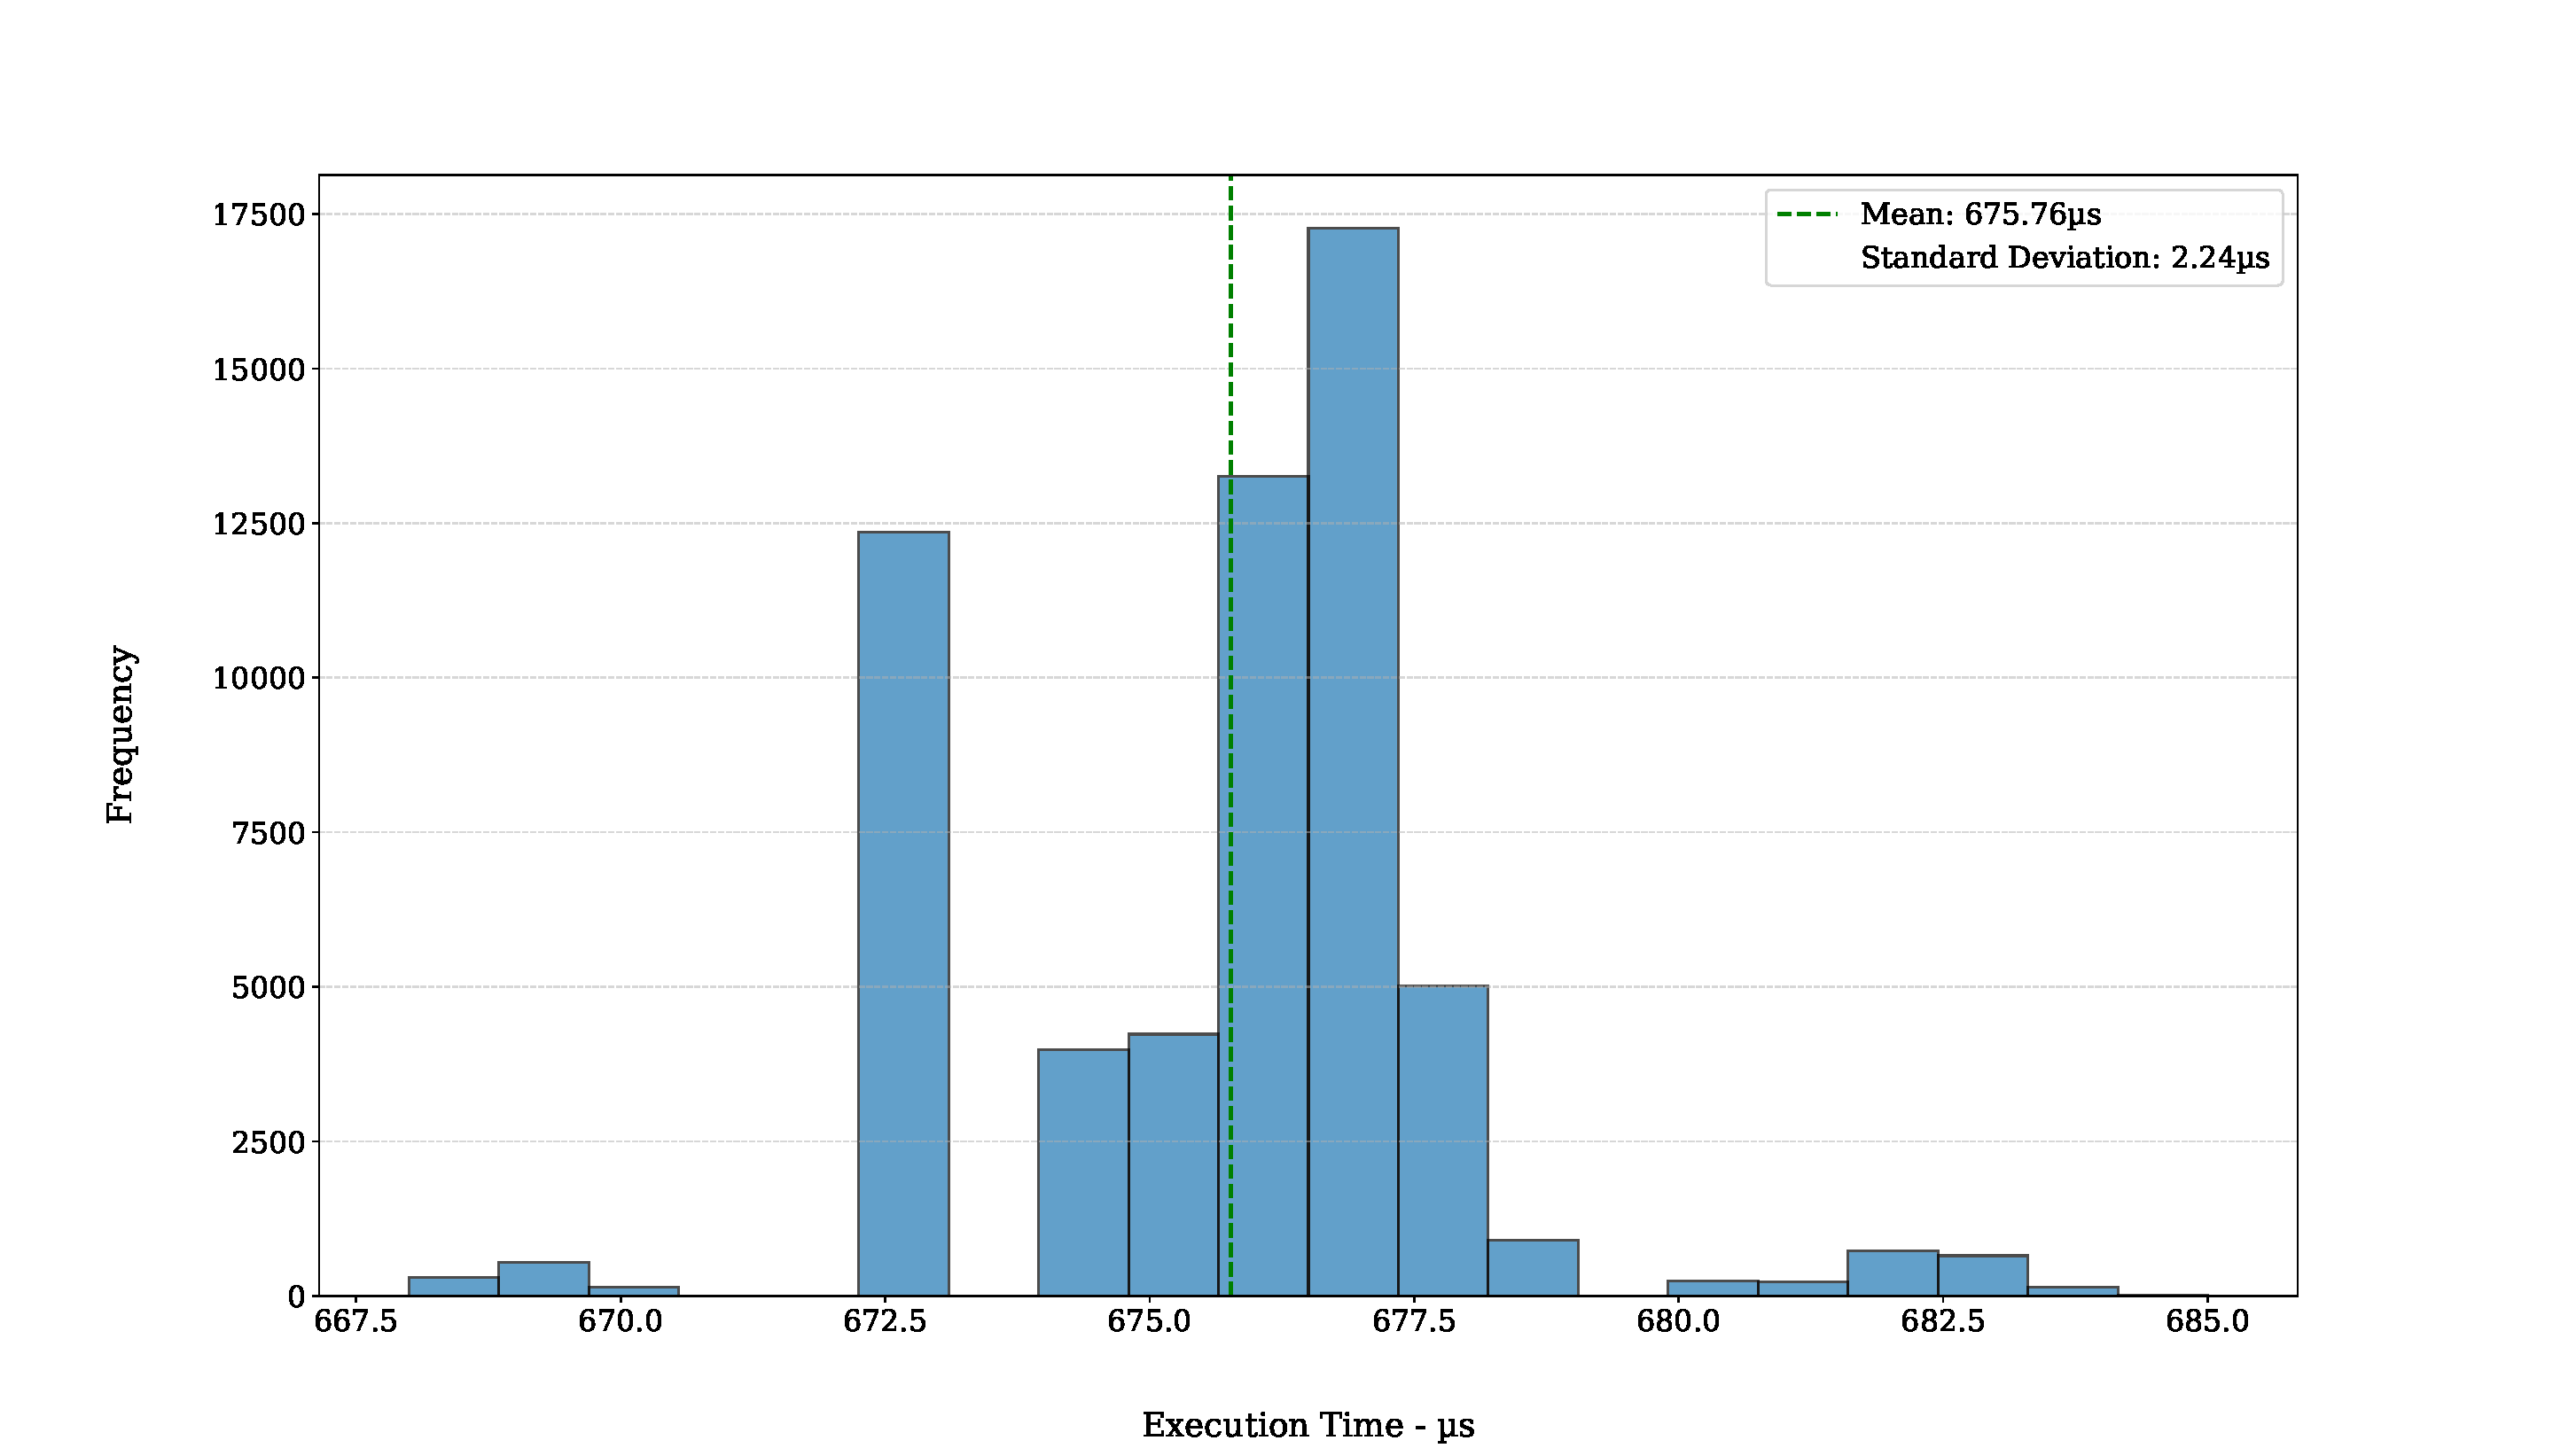
\includegraphics[width=0.95\textwidth]{images/16_without_linux.pdf}
	\caption{Tempos de Execução Das Iterações de Uma \gls{vm} Com Carga em CPU - Sem Linux.}
    \label{fig:16_without_linux}
\end{figure}

\begin{figure}[ht]
    \centering
    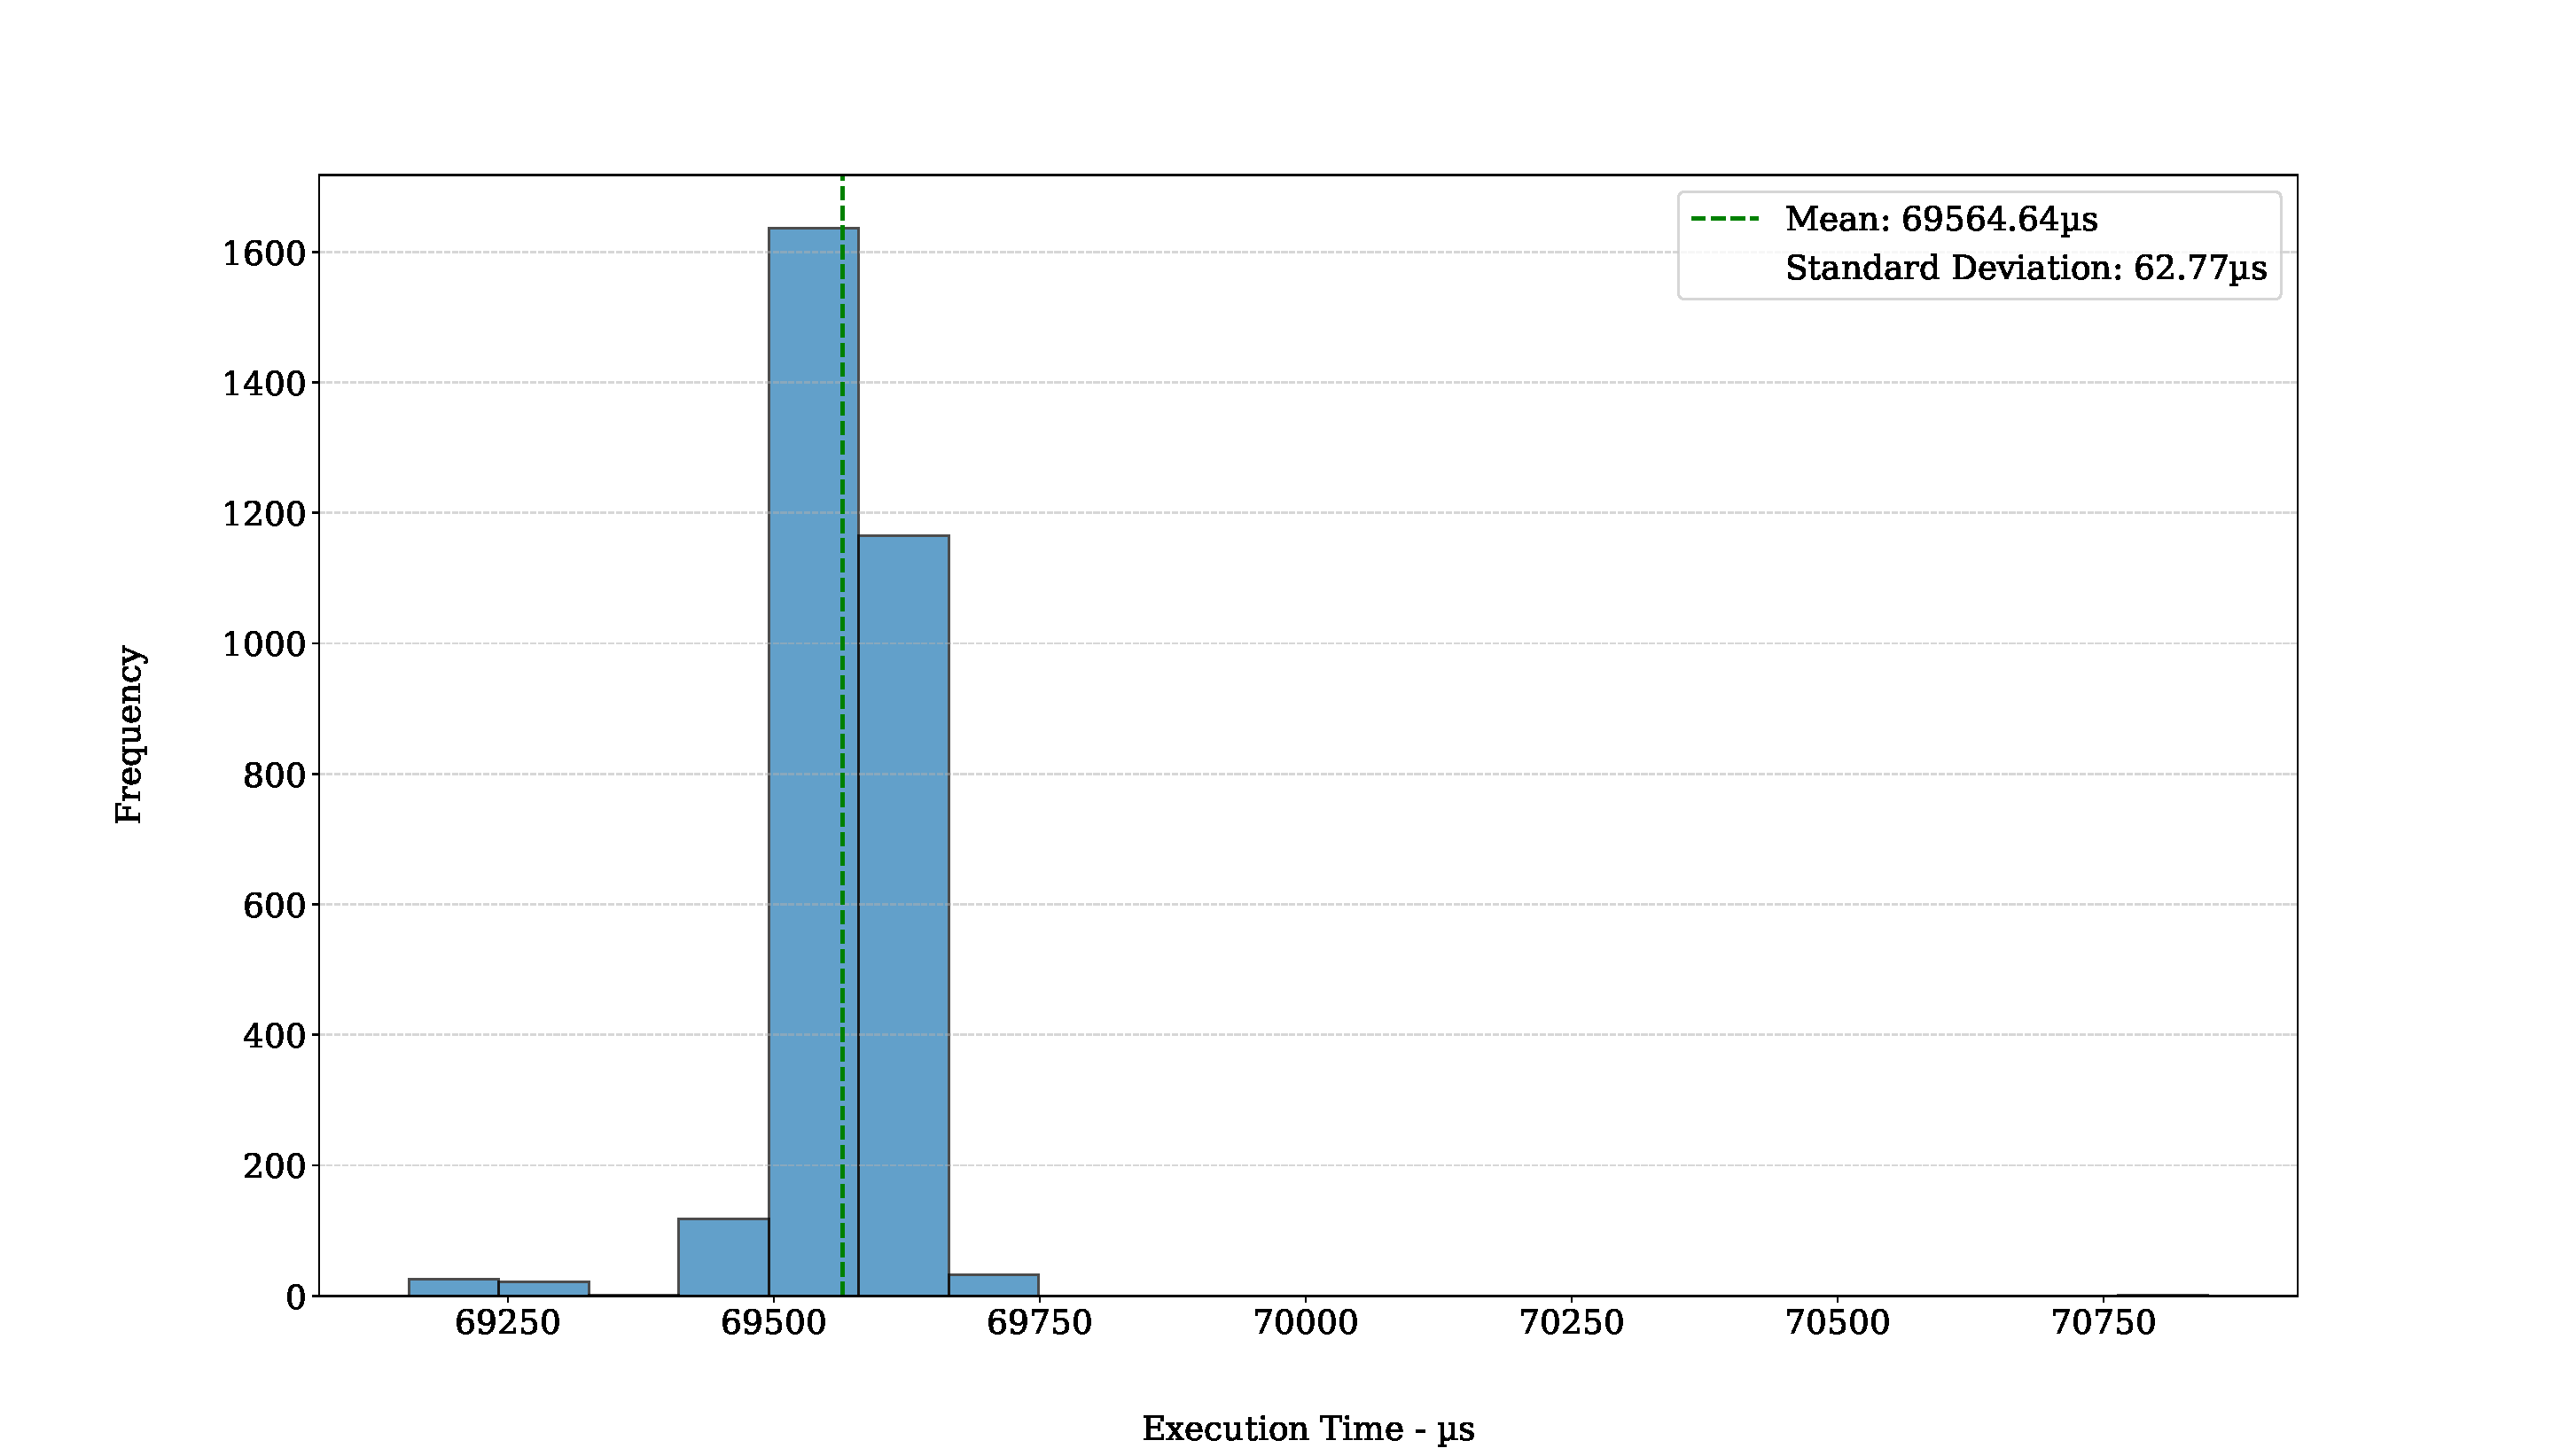
\includegraphics[width=0.95\textwidth]{images/23_without_linux.pdf}
	\caption{Tempos de Execução Das Iterações de Uma \gls{vm} Com Carga em Memória - Sem Linux.}
    \label{fig:23_without_linux}
\end{figure}

\begin{figure}[ht]
    \centering
    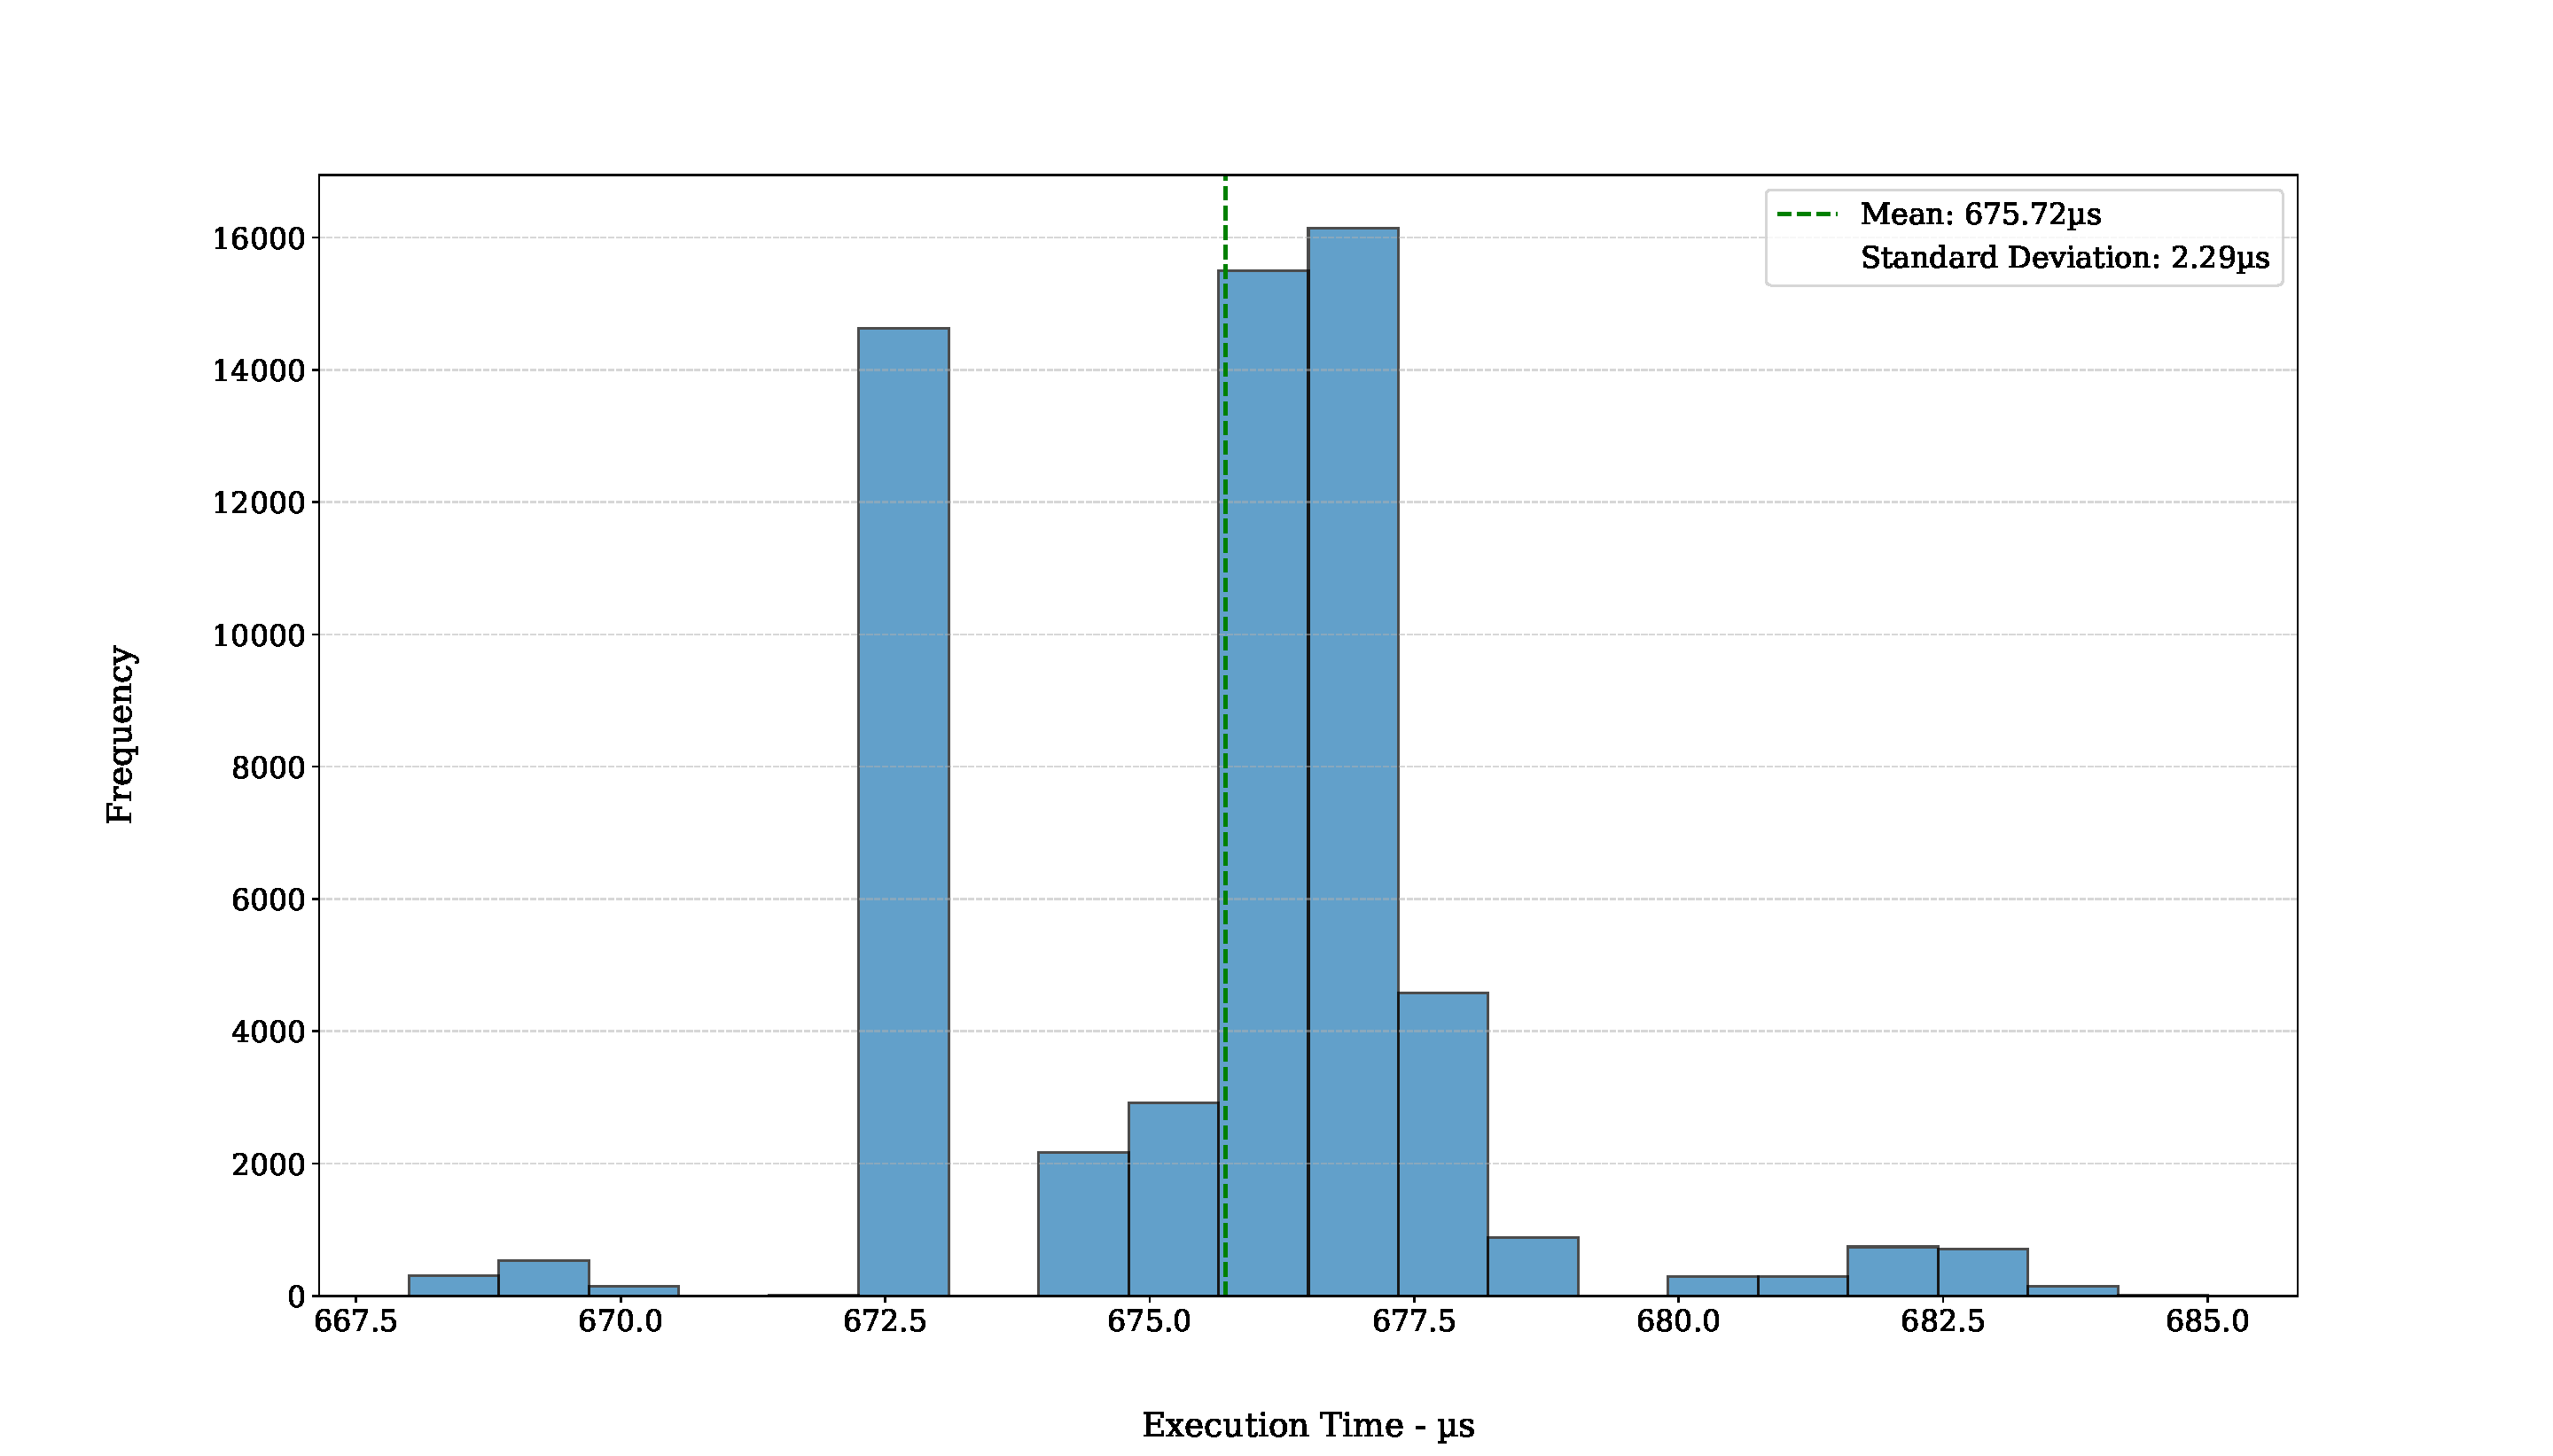
\includegraphics[width=0.95\textwidth]{images/16_with_linux.pdf}
	\caption{Tempos de Execução Das Iterações de Uma \gls{vm} Com Carga em CPU - Com Linux.}
    \label{fig:16_with_linux}
\end{figure}

\begin{figure}[ht]
    \centering
    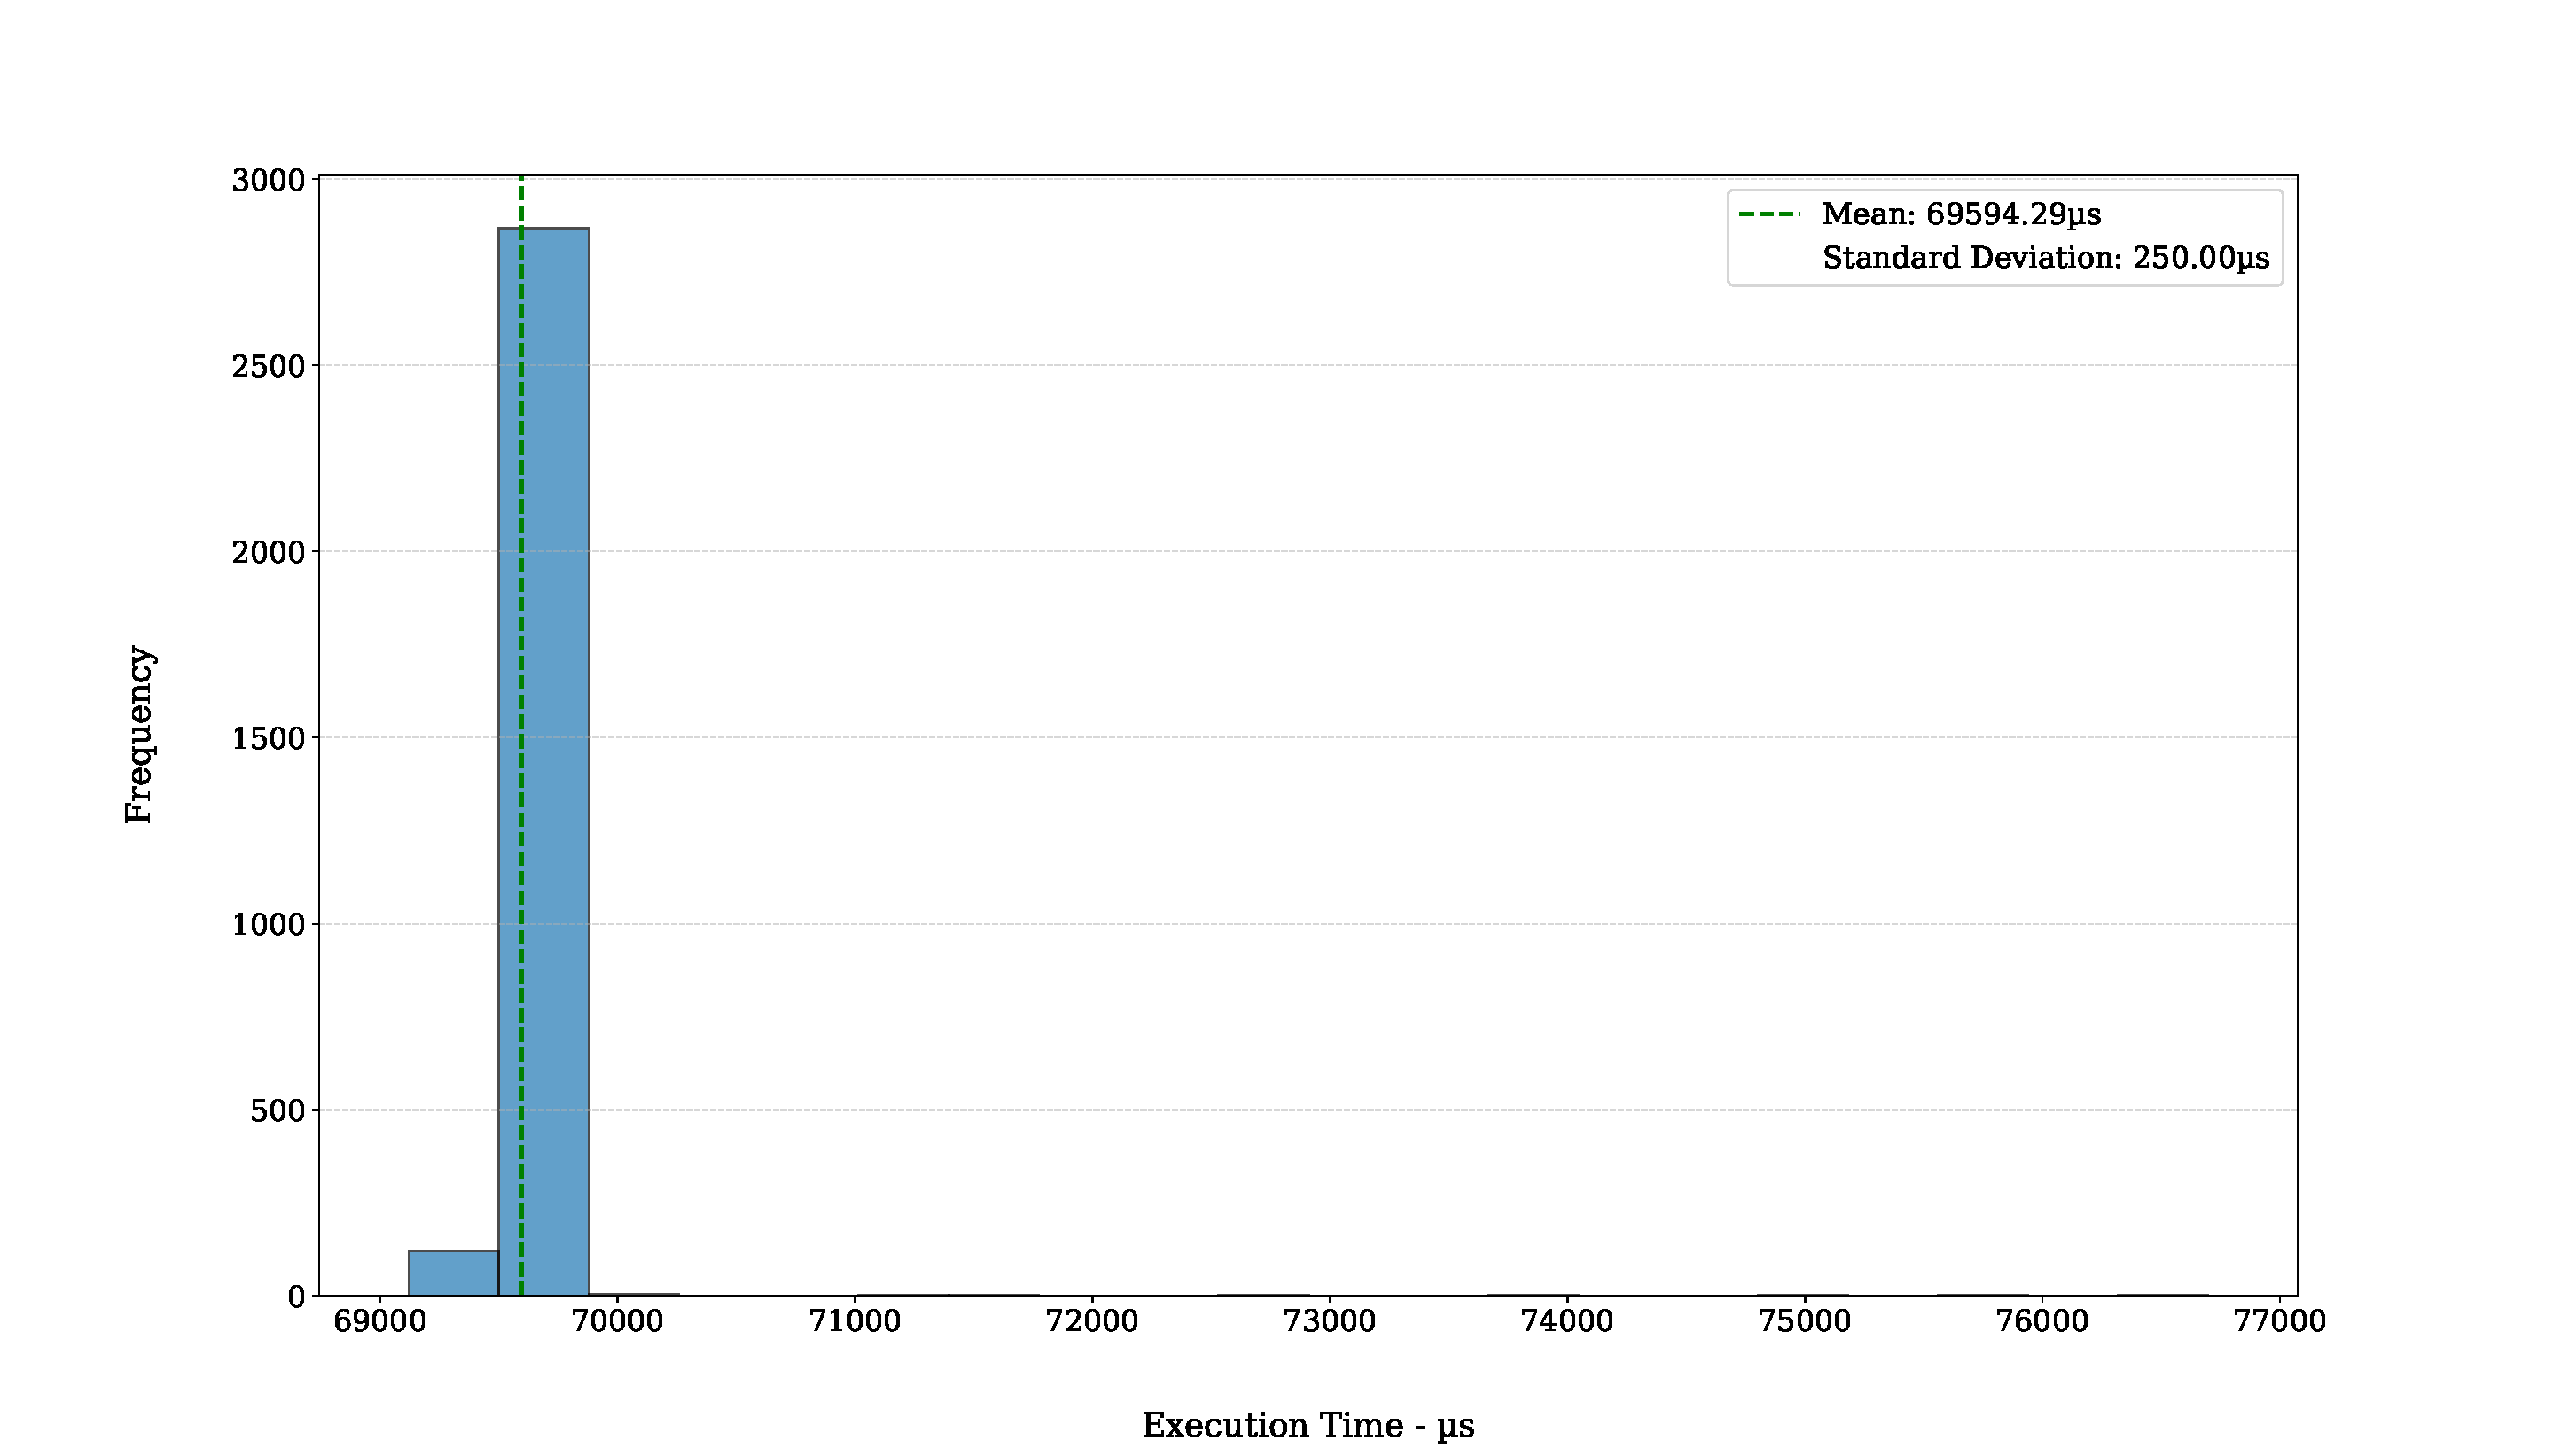
\includegraphics[width=0.95\textwidth]{images/23_with_linux.pdf}
	\caption{Tempos de Execução Das Iterações de Uma \gls{vm} Com Carga em Memória - Com Linux.}
    \label{fig:23_with_linux}
\end{figure}


\begin{figure}[ht]
    \centering
    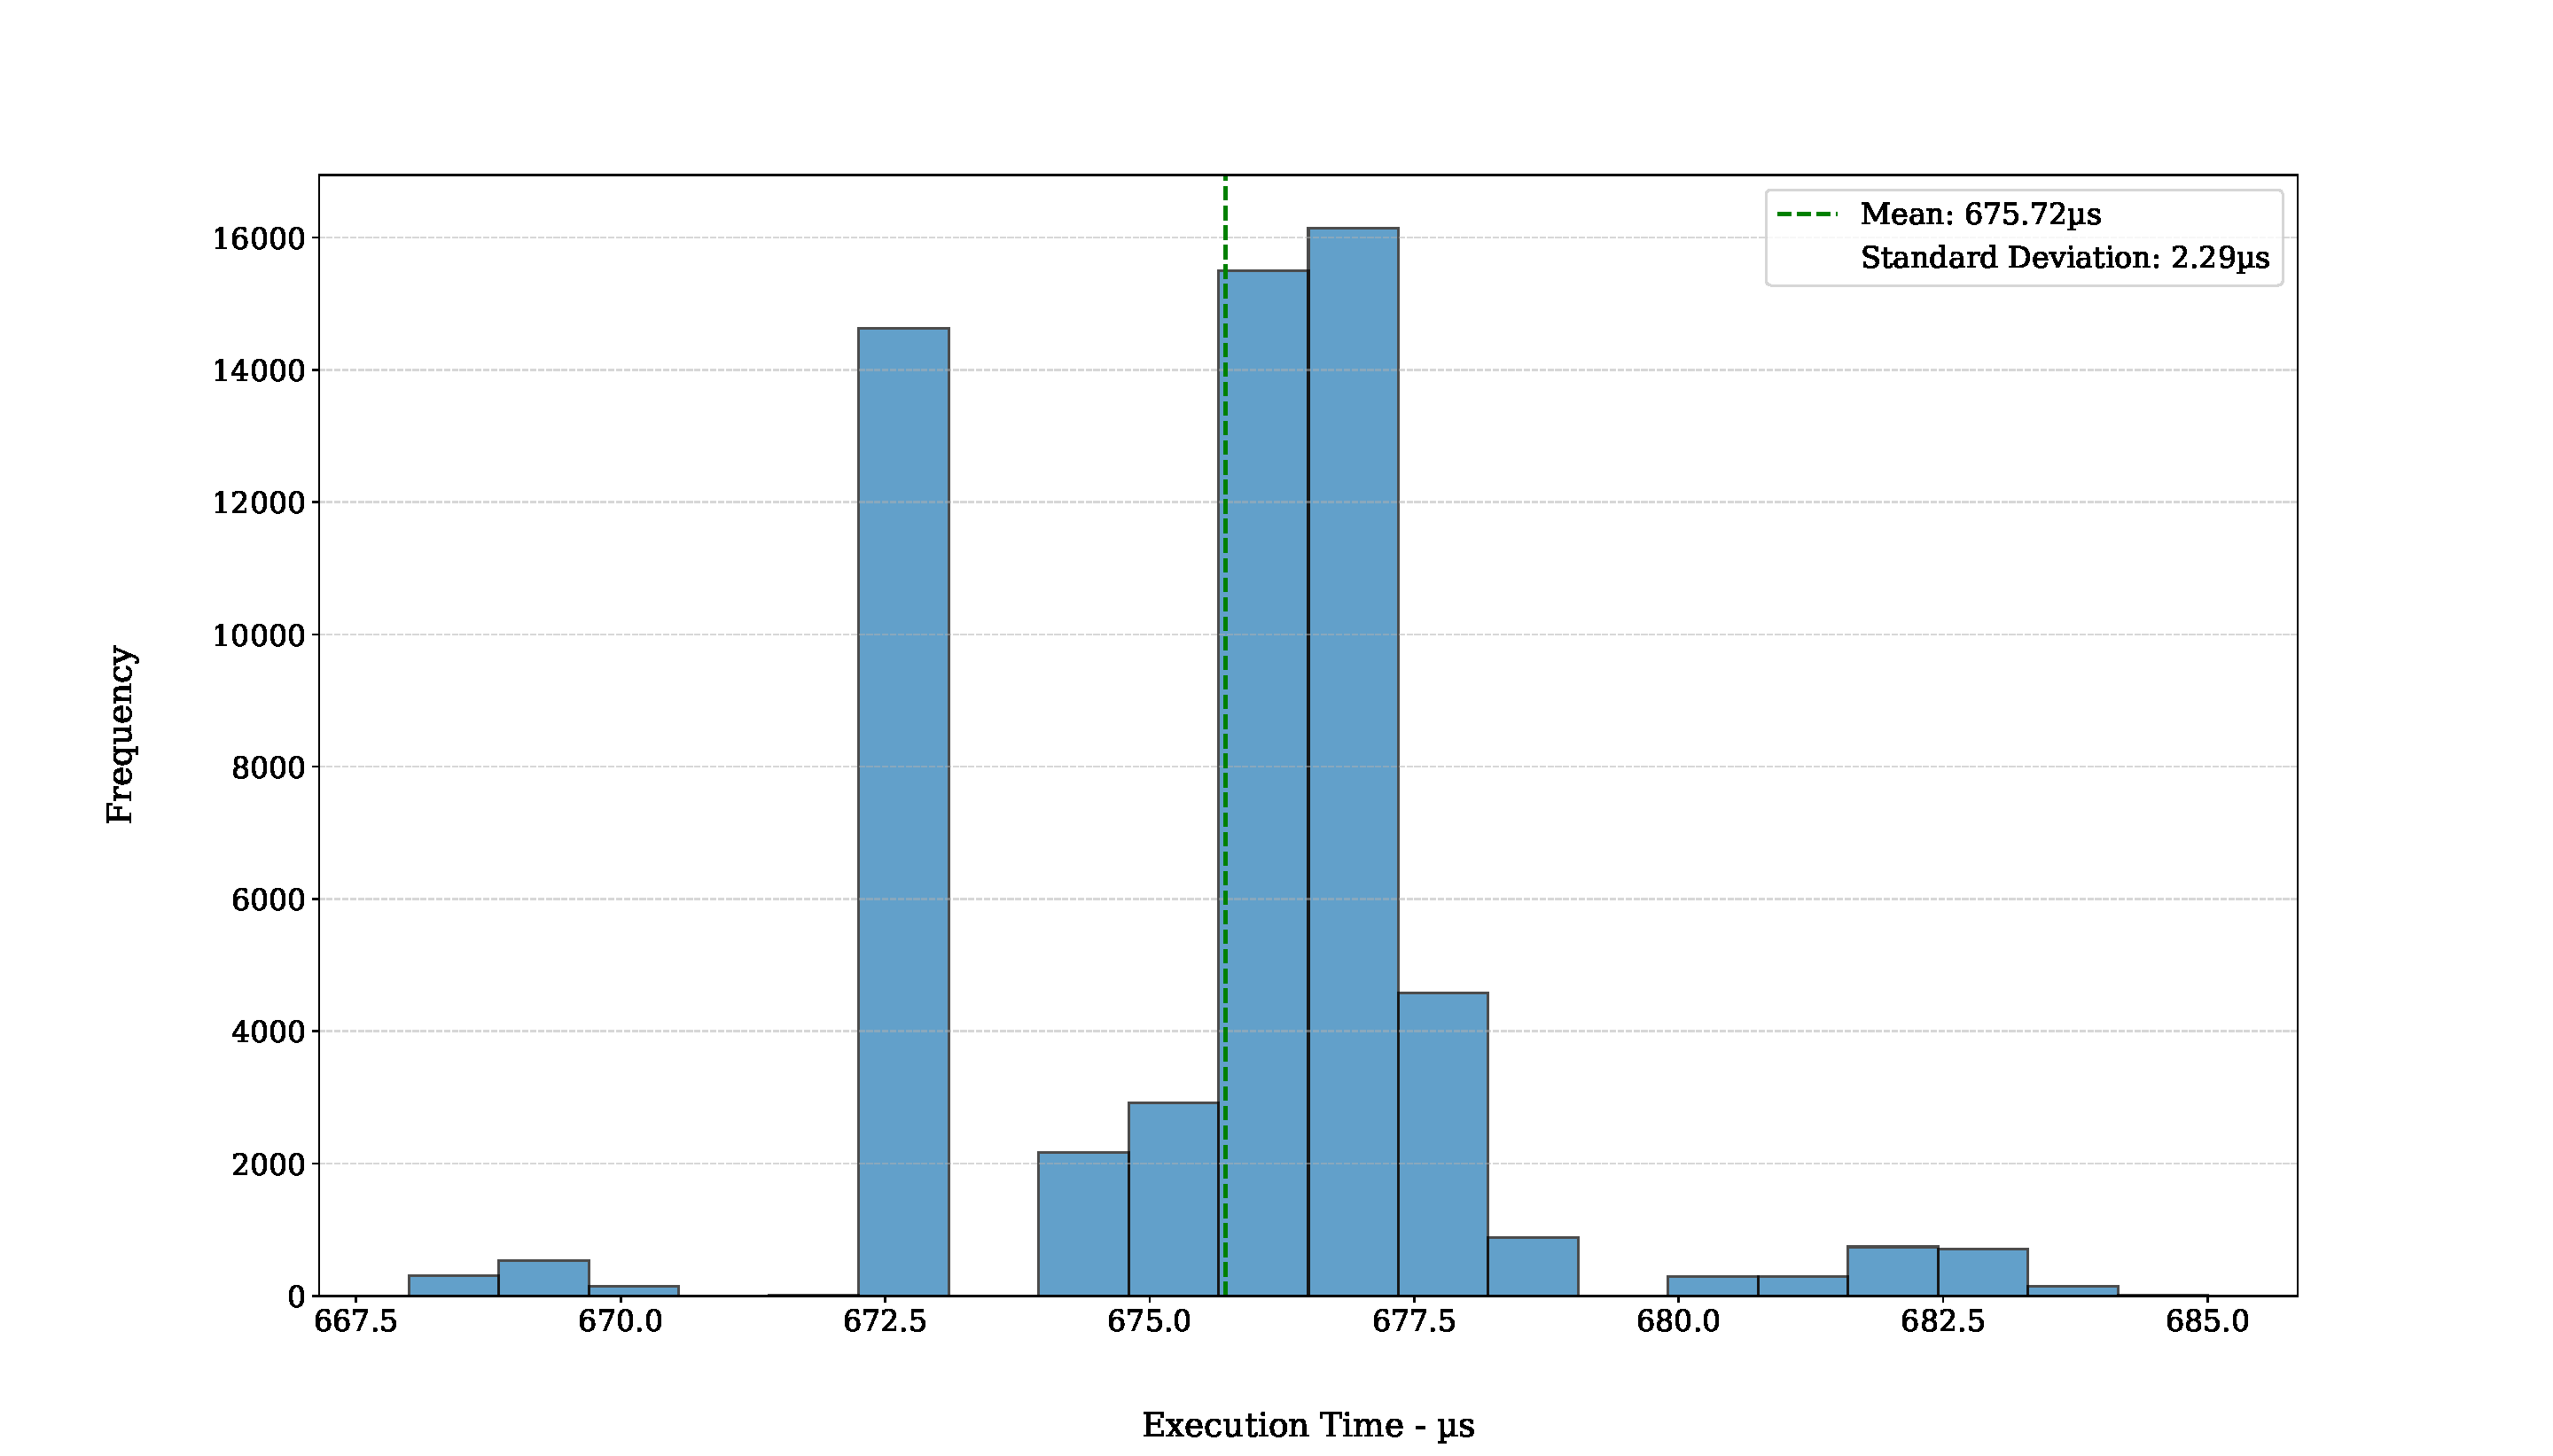
\includegraphics[width=0.95\textwidth]{images/16_with_linux_bandwidth.pdf}
	\caption{Tempos de Execução Das Iterações de Uma \gls{vm} Com Carga em CPU - Com Linux Invalidando Cache.}
    \label{fig:16_with_linux_bandwidth}
\end{figure}

\begin{figure}[ht]
    \centering
    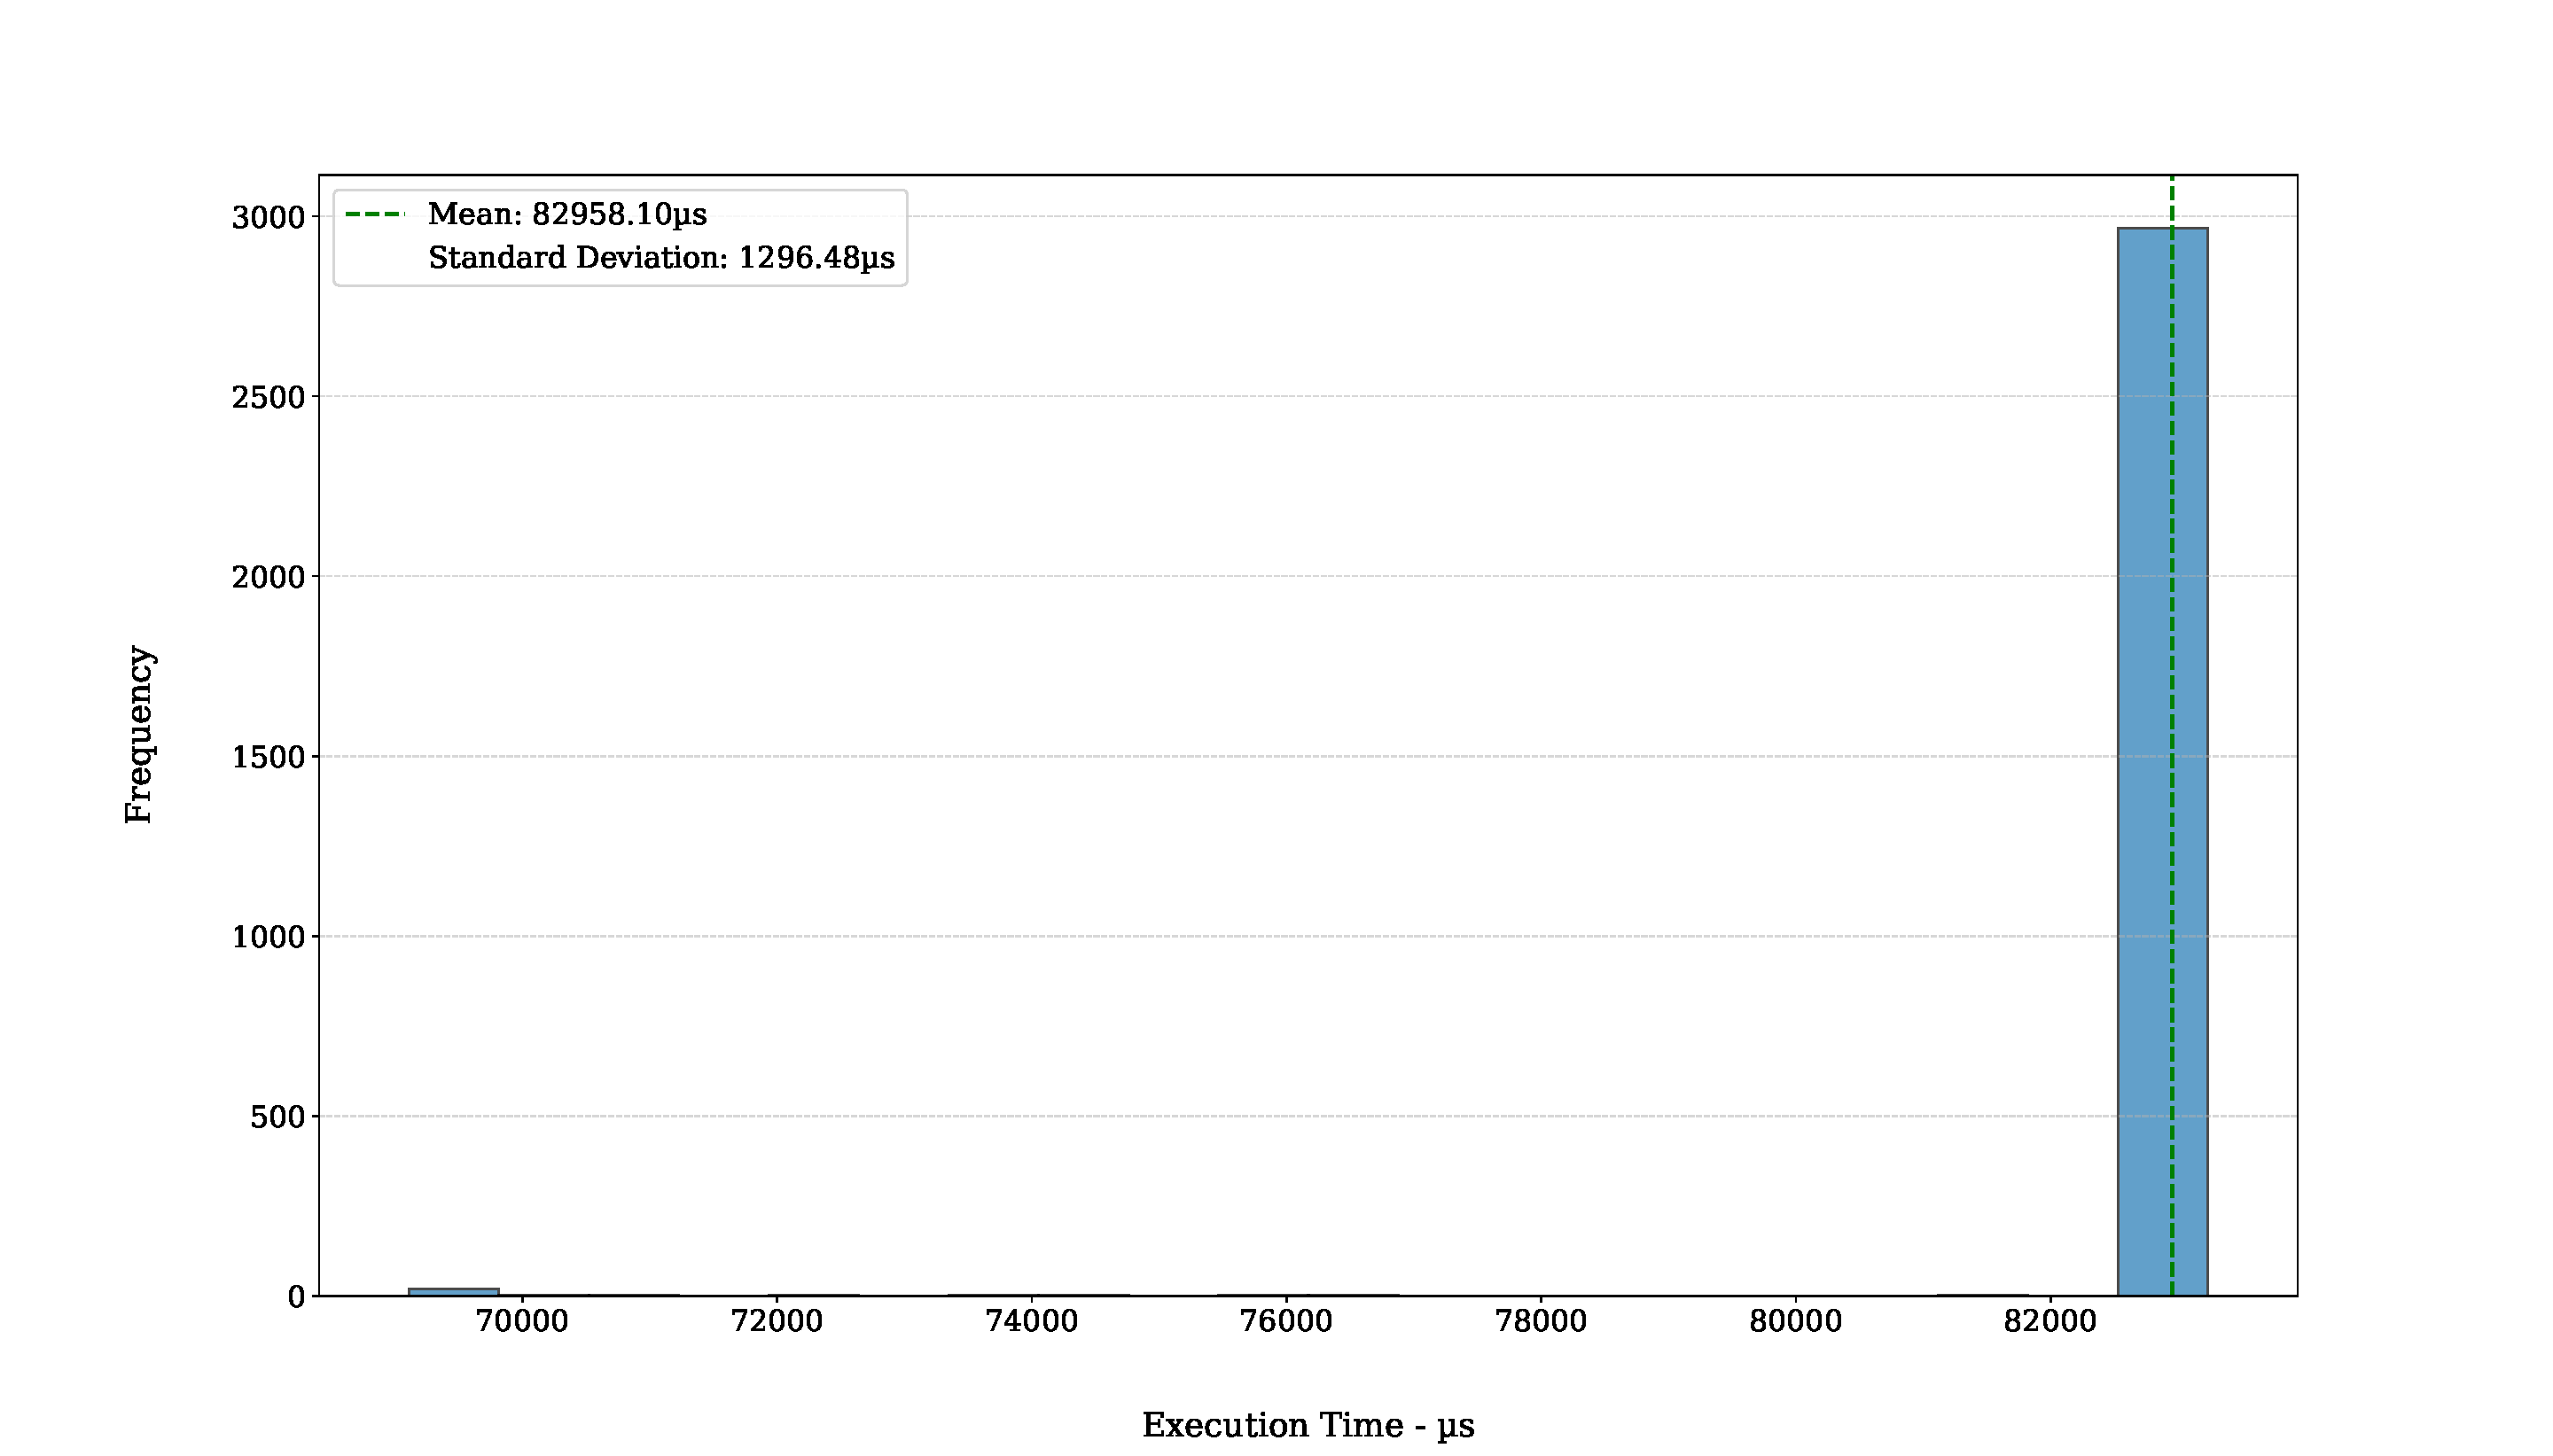
\includegraphics[width=0.95\textwidth]{images/23_with_linux_bandwidth.pdf}
	\caption{Tempos de Execução Das Iterações de Uma \gls{vm} Com Carga em Memória - Com Linux Invalidando Cache.}
    \label{fig:23_with_linux_bandwidth}
\end{figure}



%\chapter{Fundamentação Teórica}

\section{EPOS}

\gls{epos} \citeonline{EPOSPaper} é um \gls{rtos} orientado a objetos desenvolvido em C++ com foco em aplicações embarcadas e sistemas dedicados.
Sua arquitetura é baseada em componentes modulares, permitindo que apenas os recursos necessários para cada aplicação sejam incluídos no sistema final,
reduzindo consumo de memória e overhead.

O EPOS adota o conceito de \textit{Application-Oriented Operating System}, no qual o sistema operacional é configurado de acordo com os
requisitos específicos da aplicação utilizando técnicas de orientação a objetos e metaprogramação.

O trabalho desenvolvido neste documento baseia-se nos princípios arquiteturais do EPOS, especialmente em sua modularidade e abstrações.

\section{Virtualização}

Para computação, virtualização é a inserção de uma camada adicional entre um \gls{mediador-de-hardware} e o \gls{hardware} físico. Quando um componente é virtualizado,
esse recurso específico deixa de ser utilizado de forma direta e passa a ser apresentado por meio de uma abstração lógica controlada por essa camada intermediária.
Isso permite, por exemplo, que múltiplas aplicações utilizem simultaneamente o mesmo recurso, pois a camada de virtualização fica responsável por arbitrar o acesso
e coordenar seu compartilhamento evitando conflitos.

\section{Hipervisor}
Enquanto \Glspl{so} tradicionalmente atuam como supervisores (\autoref{fig:niveis-privilegio}), um hipervisor introduz uma camada adicional de abstração.
Ele opera um nível de privilégio abaixo dos \glspl{so} convidados, bloqueando o acesso direto deles ao hardware e virtualizando os recursos físicos para
orquestrar múltiplos \glspl{so} de forma isolada.

Para que essa estrutura funcione, o hipervisor utiliza mecanismos de interceptação. Como o \gls{so} convidado opera acreditando deter o privilégio máximo
sobre a máquina, ele tenta executar instruções privilegiadas diretamente. No entanto, como ele não possui esse controle essas ações geram
uma exceções que são capturadas pelo hipervisor. Este, por sua vez, traduz ou emula a operação, garantindo que o acesso aos recursos físicos ocorra
de forma segura e isolada.

Fundamentalmente, existem dois tipos de hipervisors: 1 e 2.

\subsection{Tipo 1}

Hipervisores de tipo 1, também conhecidos como bare-metal, são aqueles que executam diretamente sobre o hardware físico, sem a necessidade de um
sistema operacional hospedeiro intermediário. Eles atuam como \gls{so} e como camada de virtualização apresentando maior desempenho e menor latência
em comparação aos hipervisores do Tipo 2. Além disso, proporcionam maior controle sobre os recursos do sistema e melhor isolamento entre as máquinas virtuais,
tornando-os especialmente adequados para ambientes críticos.

\begin{figure}[htbp]
    \centering
    \begin{tikzpicture}[
        pequeno/.style={
            draw,
            thick,
            fill=blue!5,
            minimum width=4cm,
            minimum height=1.2cm,
            outer sep=0pt
        }
    ]
        \node[pequeno] (apps-so1-1) {Aplicação 1};
        \node[pequeno, right=0.2cm of apps-so1-1] (apps-so1-2) {Aplicação 2};
        \node[pequeno, right=0.2cm of apps-so1-2] (apps-so2-1) {Aplicação 1};

        \node[fit=(apps-so1-1)(apps-so1-2), inner sep=0pt] (apps-so1) {};
        \node[fit=(apps-so2-1), inner sep=0pt] (apps-so2) {};

        \node[
            draw,
            thick,
            fill=blue!10,
            minimum width=8.2cm,
            minimum height=1.5cm,
            below=0.2cm of apps-so1
		] (SO1) {\Gls{so} 1};

		\node[
            draw,
            thick,
            fill=blue!10,
            minimum width=4cm,
            minimum height=1.5cm,
            below=0.2cm of apps-so2
		] (SO2) {\Gls{so} 2};

		\node[fit=(SO2)(SO1), inner sep=0pt] (SOs) {};

		\node[
            draw,
            thick,
            fill=blue!15,
            minimum width=12.4cm,
            minimum height=1.5cm,
            below=0.2cm of SOs
		] (HOS) {Hipervisor};

		\node[
            draw,
            thick,
            fill=blue!20,
            minimum width=12.4cm,
            minimum height=1.5cm,
            below=0.2cm of HOS
		] () {\Gls{hardware}};

    \end{tikzpicture}
    \caption{Hipervisor Tipo 1.}
    \label{fig:hypervisor-type-1}
\end{figure}

\subsection{Tipo 2}

Diferentemente da solução nativa, um hipervisor de Tipo 2 é executado como um processo dentro de um \gls{so} hospedeiro.
Apesar de garantir o isolamento e a virtualização para diversos \glspl{so} convidados, sua arquitetura impõe mais uma camada intermediária de
software que restringe a eficiência no acesso aos componentes físicos, gerando latência adicional e menor desempenho em operações críticas.

\begin{figure}[htbp]
    \centering
    \begin{tikzpicture}[
        pequeno/.style={
            draw,
            thick,
            fill=blue!5,
            minimum width=4cm,
            minimum height=1.2cm,
            outer sep=0pt
        }
    ]
        \node[pequeno] (apps-so1-1) {Aplicação 1};
        \node[pequeno, right=0.2cm of apps-so1-1] (apps-so1-2) {Aplicação 2};
        \node[pequeno, right=0.2cm of apps-so1-2] (apps-so2-1) {Aplicação 1};

        \node[fit=(apps-so1-1)(apps-so1-2), inner sep=0pt] (apps-so1) {};
        \node[fit=(apps-so2-1), inner sep=0pt] (apps-so2) {};

        \node[
            draw,
            thick,
            fill=blue!10,
            minimum width=8.2cm,
            minimum height=1.5cm,
            below=0.2cm of apps-so1
		] (SO1) {\Gls{so} 1};

		\node[
            draw,
            thick,
            fill=blue!10,
            minimum width=4cm,
            minimum height=1.5cm,
            below=0.2cm of apps-so2
		] (SO2) {\Gls{so} 2};

		\node[fit=(SO2)(SO1), inner sep=0pt] (SOs) {};

		\node[
            draw,
            thick,
            fill=blue!15,
            minimum width=12.4cm,
            minimum height=1.5cm,
            below=0.2cm of SOs
		] (HOS) {Hipervisor};

		\node[
            draw,
            thick,
            fill=blue!20,
            minimum width=12.4cm,
            minimum height=1.5cm,
            below=0.2cm of HOS
		] (OS) {\Gls{so}};

		\node[
            draw,
            thick,
            fill=blue!25,
            minimum width=12.4cm,
            minimum height=1.5cm,
            below=0.2cm of OS
		] () {\Gls{hardware}};

    \end{tikzpicture}
    \caption{Hipervisor Tipo 2.}
    \label{fig:hypervisor-type-2}
\end{figure}




\section{Interceptação e Emulação - Trap and Emulate}




\section{Hipervisors}

Um hipervisor, também conhecido como \gls{vmm}, é uma plataforma que cria e executa máquinas virtuais via virtualização.
Segundo \citeonline{PopekGeraldGoldberg} um \gls{vmm} possuí três características essenciais: primeiro, devem fornecer um ambiente idêntico à máquina original
para programas; segundo, os programas executados nesse ambiente, na pior das hipóteses, devem apresentar no máximo pequenas reduções
de velocidade que urgem da camada de virtualização; e por último, os \glspl{vmm} devem deter o contole total sobre os recursos do sistema.

Na visão de \cite{Goldberg}, fundamentalmente, existem dois tipos de hipervisores: 1 e 2.

\subsection{Tipo 1 - Bare Metal}

Hipervisores de tipo 1, também conhecidos como bare metal, são aqueles que executam diretamente sobre o hardware físico, sem a necessidade de um
sistema operacional hospedeiro intermediário.
Por operar diretamente sobre o hardware, esse tipo de hipervisor geralmente apresenta melhor desempenho e menor sobrecarga.

\begin{figure}[H]
    \centering
    \begin{tikzpicture}[
        pequeno/.style={
            draw,
            thick,
            fill=blue!5,
            minimum width=4cm,
            minimum height=1.2cm,
            outer sep=0pt
        }
    ]
        \node[pequeno] (apps-so1-1) {Aplicação 1};
        \node[pequeno, right=0.2cm of apps-so1-1] (apps-so1-2) {Aplicação 2};
        \node[pequeno, right=0.2cm of apps-so1-2] (apps-so2-1) {Aplicação 1};

        \node[fit=(apps-so1-1)(apps-so1-2), inner sep=0pt] (apps-so1) {};
        \node[fit=(apps-so2-1), inner sep=0pt] (apps-so2) {};

        \node[
            draw,
            thick,
            fill=blue!10,
            minimum width=8.2cm,
            minimum height=1.5cm,
            below=0.2cm of apps-so1
		] (SO1) {\Gls{so} 1};

		\node[
            draw,
            thick,
            fill=blue!10,
            minimum width=4cm,
            minimum height=1.5cm,
            below=0.2cm of apps-so2
		] (SO2) {\Gls{so} 2};

		\node[fit=(SO2)(SO1), inner sep=0pt] (SOs) {};

		\node[
            draw,
            thick,
            fill=blue!15,
            minimum width=12.4cm,
            minimum height=1.5cm,
            below=0.2cm of SOs
		] (HOS) {Hipervisor};

		\node[
            draw,
            thick,
            fill=blue!20,
            minimum width=12.4cm,
            minimum height=1.5cm,
            below=0.2cm of HOS
		] () {Hardware};

    \end{tikzpicture}
    \caption{Hipervisor Tipo 1.}
    \label{fig:hypervisor-type-1}
\end{figure}

\subsection{Tipo 2}

Diferentemente da solução bare metal, um hipervisor do tipo 2 é executado como um processo dentro de um \gls{so} hospedeiro.
Porém, apesar de garantir os mesmos recursos do tipo 1, sua arquitetura impõe uma camada intermediária a mais de software, o que restringe a
eficiência no acesso aos componentes físicos, gerando uma latência adicional e um menor desempenho.

\begin{figure}[H]
    \centering
    \begin{tikzpicture}[
        pequeno/.style={
            draw,
            thick,
            fill=blue!5,
            minimum width=4cm,
            minimum height=1.2cm,
            outer sep=0pt
        }
    ]
        \node[pequeno] (apps-so1-1) {Aplicação 1};
        \node[pequeno, right=0.2cm of apps-so1-1] (apps-so1-2) {Aplicação 2};
        \node[pequeno, right=0.2cm of apps-so1-2] (apps-so2-1) {Aplicação 1};

        \node[fit=(apps-so1-1)(apps-so1-2), inner sep=0pt] (apps-so1) {};
        \node[fit=(apps-so2-1), inner sep=0pt] (apps-so2) {};

        \node[
            draw,
            thick,
            fill=blue!10,
            minimum width=8.2cm,
            minimum height=1.5cm,
            below=0.2cm of apps-so1
		] (SO1) {\Gls{so} 1};

		\node[
            draw,
            thick,
            fill=blue!10,
            minimum width=4cm,
            minimum height=1.5cm,
            below=0.2cm of apps-so2
		] (SO2) {\Gls{so} 2};

		\node[fit=(SO2)(SO1), inner sep=0pt] (SOs) {};

		\node[
            draw,
            thick,
            fill=blue!15,
            minimum width=12.4cm,
            minimum height=1.5cm,
            below=0.2cm of SOs
		] (HOS) {Hipervisor};

		\node[
            draw,
            thick,
            fill=blue!20,
            minimum width=12.4cm,
            minimum height=1.5cm,
            below=0.2cm of HOS
		] (OS) {\Gls{so}};

		\node[
            draw,
            thick,
            fill=blue!25,
            minimum width=12.4cm,
            minimum height=1.5cm,
            below=0.2cm of OS
		] () {Hardware};

    \end{tikzpicture}
    \caption{Hipervisor Tipo 2.}
    \label{fig:hypervisor-type-2}
\end{figure}

\section{Diferenças Entre Virtualização e Emulação}

Algumas funcionalidades utilizadas neste trabalho serão emuladas em vez de virtualizadas, devido a limitações de hardware.
A principal diferença entre esses dois conceitos está na forma como as operações são executadas.

A emulação é realizada inteiramente por software, reproduzindo o comportamento de uma arquitetura ou dispositivo por meio da interpretação ou tradução
de instruções. Entretanto, devido à necessidade de traduzir instruções e simular componentes de hardware, a emulação tende a apresentar menor desempenho
em relação a virtualização.

Por outro lado, embora a virtualização também introduza uma camada de software, esta atua primariamente como uma interface de controle e gerenciamento.
Isso permite que a maior parte das instruções seja executada diretamente pelo processador físico. Contudo, essa abordagem exige suporte especializado
por parte do hardware subjacente, um requisito que nem sempre está disponível em todas as arquiteturas e máquinas.

\section{RISC-V}

O RISC-V é uma \gls{isa} baseada nos princípios da arquitetura \acrshort{risc} (\acrlong{risc}). Diferentemente de arquiteturas proprietárias,
o RISC-V possui uma especificação aberta e livre de royalties, o que permite sua utilização tanto em contextos acadêmicos quanto em aplicações
comerciais.

Essa \gls{isa} define um conjunto básico de instruções, responsável pelas funcionalidades essenciais do processador. No entanto, sua
principal característica é a modularidade, permitindo que diferentes extensões sejam incorporadas conforme as necessidades da aplicação.
Dessa forma, é possível adaptar a arquitetura para cenários variados, desde sistemas embarcados com restrições de recursos até sistemas de
alto desempenho.

\subsection{Extensões}

\begin{description}

\item[I]
Instruções básicas para operações com números inteiros. Conforme descrito em \cite{RISCVUnprivilegedISA}, essa extensão deve estar presente em
qualquer implementação RISC-V, pois define operações fundamentais de aritmética e manipulação de registradores.

\item[Zicsr]
Adiciona suporte às instruções de acesso e manipulação de \glspl{csr}.

\item[H]
Adiciona suporte em hardware à virtualização. Porém, apesar de existir, é muito recente e sua implementação em hardware comercial ainda é limitada.

\item[M]
Adiciona suporte à operações de multiplicação e divisão de números inteiros.

\item[A]
Adiciona suporte à operações atômicas em memória.

\item[F]
Adiciona suporte a números em ponto flutuante de precisão simples (32 bits).

\item[D]
Adiciona suporte a números em ponto flutuante de precisão dupla (64 bits).

\item[C]
Adiciona suporte à instruções comprimidas de 16 bits.

\item[S]
Adiciona suporte ao modo supervisor.

\item[G]
Aglomerado geral de extensões que inclui I, M, A, F, D e C.

\end{description}

Para o escopo deste trabalho, serão consideradas apenas as extensões Zicsr, S e G. As estratégias adotadas para mitigar a ausência da extensão H
serão discutidas ao longo do texto.

\subsection{Níveis de Privilégio}
\subsection{Control and Status Registers (CSRs)}

\section{Interceptação e Emulação}

Do inglês \textit{trap-and-emulate}, interceptação e emulação trata-se de um método utilizado para viabilizar a virtualização em sistemas nos quais o suporte de hardware não é completamente implementado.
Nesse modelo, quando a aplicação executada em ambiente virtualizado tenta realizar uma operação que depende de recursos privilegiados, essa operação é interceptada e tratada como uma exceção.
O controle é então transferido para um nível de privilégio superior, geralmente o hipervisor, que fica responsável por emular em software o comportamento esperado da instrução ou operação originalmente solicitada.

\section{\textit{VirtIO}}

O \textit{VirtIO} \cite{RustyRussellVirtIO} é um modelo de dispositivo virtual projetado para padronizar a comunicação de operações de \gls{io} entre \glspl{so} convidados e seus respectivos hipervisores.
Seu funcionamento assemelha-se ao de dispositivos físicos baseados em \gls{dma}, empregando regiões de memória compartilhada para a transferência direta de dados.

Para viabilizar essa comunicação, o modelo utiliza as chamadas \textit{Virtqueues} — filas circulares compartilhadas responsáveis pelo envio e recebimento das requisições. Dependendo das operações suportadas,
cada dispositivo virtual pode alocar uma ou mais dessas filas. Internamente, uma \textit{Virtqueue} divide-se em três componentes principais: uma tabela de descritores (\textit{Descriptor Table}), um anel de
índices disponíveis (\textit{Available Ring}) e um anel de índices já utilizados (\textit{Used Ring}).

Na prática, o ciclo de vida de uma operação de \gls{io} ocorre em duas etapas complementares. Inicialmente, quando o sistema convidado deseja realizar uma operação, o \textit{driver VirtIO} escreve os dados
na memória compartilhada, insere o descritor correspondente no \textit{Available Ring} e notifica o hipervisor sobre a nova pendência. 

Em resposta, o hipervisor consome os descritores desse anel, processa a operação solicitada e registra o resultado no \textit{Used Ring}. Por fim, uma interrupção é enviada ao sistema convidado para sinalizar a
conclusão da tarefa. Graças a esse design, múltiplas requisições podem ser tratadas de maneira assíncrona e em lote, o que minimiza as trocas de contexto e reduz expressivamente o custo inerente à virtualização.

Desse modo, o \textit{VirtIO} consolida-se como uma solução fundamental para a infraestrutura de virtualização moderna, pois alcança um equilíbrio entre a flexibilidade de uma interface padronizada e o
desempenho da paravirtualização.


%\section{Níveis de Privilégio}

Os níveis de privilégio surgem com a evolução dos \glspl{so} e com a necessidade de particionar e proteger os recursos de um computador.
Esses níveis são organizados em um modelo de camadas, no qual a camada mais alta possui acesso mais restrito, enquanto a camada mais baixa detém controle total sobre o \gls{hardware}.
Além disso, como os níveis superiores não possuem acesso direto a determinados recursos, os níveis inferiores podem lhes fornecer serviços, abstrações e mecanismos de acesso, sempre de forma controlada.
Embora a implementação desses níveis varie entre diferentes arquiteturas, não é desejável que todas as aplicações executem no nível mais privilegiado, pois isso pode comprometer o isolamento
entre processos e gerar competição descontrolada pelos recursos do sistema.
Por isso, a maioria dos processadores e \glspl{so} adotam, no mínimo, uma divisão binária com o modo usuário e o modo supervisor, ilustrados na Figura~\ref{fig:niveis-privilegio}.

\begin{figure}[htbp]
    \centering
    \begin{tikzpicture}[
        >=Stealth,
        camada/.style={
            draw,
            thick,
            minimum width=6cm,
            minimum height=1.2cm,
            outer sep=0pt
        }
    ]
        \node[camada, fill=blue!5] (u) {Usuário (U-Mode)};
        \node[camada, fill=blue!10, below=0.2cm of u] (s) {Supervisor (S-Mode)};
        \node[camada, fill=blue!15, below=0.2cm of s] (h) {\Gls{hardware}};

    \end{tikzpicture}
    \caption{Exemplo Básico de Níveis de Privilégio.}
    \label{fig:niveis-privilegio}
\end{figure}

O modo usuário é destinado à execução da maioria das aplicações. Nesse nível, os programas operam com acesso restrito aos recursos do sistema, sem executar instruções privilegiadas
nem acessar diretamente componentes críticos da máquina.

Já o modo supervisor é destinado à execução do próprio \gls{so}, dispondo de acesso total aos recursos do sistema. Nesse nível, o sistema operacional gerencia memória, dispositivos
e processos, atuando como intermediário entre os programas em modo usuário e o hardware.



%\section{\textit{VirtIO}}

O \textit{VirtIO} \cite{RustyRussellVirtIO} é um modelo de dispositivo virtual projetado para padronizar a comunicação de operações de \gls{io} entre \glspl{so} convidados e seus respectivos hipervisores.
Seu funcionamento assemelha-se ao de dispositivos físicos baseados em \gls{dma}, empregando regiões de memória compartilhada para a transferência direta de dados.

Para viabilizar essa comunicação, o modelo utiliza as chamadas \textit{Virtqueues} — filas circulares compartilhadas responsáveis pelo envio e recebimento das requisições. Dependendo das operações suportadas,
cada dispositivo virtual pode alocar uma ou mais dessas filas. Internamente, uma \textit{Virtqueue} divide-se em três componentes principais: uma tabela de descritores (\textit{Descriptor Table}), um anel de
índices disponíveis (\textit{Available Ring}) e um anel de índices já utilizados (\textit{Used Ring}).

Na prática, o ciclo de vida de uma operação de \gls{io} ocorre em duas etapas complementares. Inicialmente, quando o sistema convidado deseja realizar uma operação, o \textit{driver VirtIO} escreve os dados
na memória compartilhada, insere o descritor correspondente no \textit{Available Ring} e notifica o hipervisor sobre a nova pendência. 

Em resposta, o hipervisor consome os descritores desse anel, processa a operação solicitada e registra o resultado no \textit{Used Ring}. Por fim, uma interrupção é enviada ao sistema convidado para sinalizar a
conclusão da tarefa. Graças a esse design, múltiplas requisições podem ser tratadas de maneira assíncrona e em lote, o que minimiza as trocas de contexto e reduz expressivamente o custo inerente à virtualização.

Desse modo, o \textit{VirtIO} consolida-se como uma solução fundamental para a infraestrutura de virtualização moderna, pois alcança um equilíbrio entre a flexibilidade de uma interface padronizada e o
desempenho da paravirtualização.



% Hypervisors
% Trap-and-Emulate Hypervisors
% Passthrough Devices
% VirtIO 

%\chapter{Metodologia}

\section{Virtualização Baseada em Modo Máquina}

O \textit{Machine Mode} foi concebido originalmente na arquitetura RISC-V como o nível de privilégio mais elevado, responsável pela execução do firmware base e pelo controle direto dos recursos de hardware.
O software residente nesse nível encarrega-se da inicialização da plataforma, da configuração dos subsistemas fundamentais e, subsequentemente, da transferência de controle para o \gls{so} hospedeiro. 

Além das responsabilidades de inicialização, determinadas implementações da arquitetura requerem que o modo máquina forneça serviços privilegiados às camadas superiores. Esses serviços são disponibilizados
por meio de interfaces padronizadas, como a \gls{sbi}, permitindo que sistemas executados em níveis menos privilegiados acessem de forma controlada as funcionalidades de hardware restritas.

No escopo deste trabalho, o M-mode é empregado de forma atípica: como a camada base para a implementação de um hipervisor, visando contornar a ausência da extensão de virtualização (H) na plataforma utilizada.
Esta estratégia fundamenta-se na autoridade irrestrita que o modo máquina possui sobre os demais níveis de privilégio da arquitetura, o que viabiliza o controle e a orquestração integral dos \glspl{so} convidados.
Para tanto, o M-mode dispõe de um conjunto isolado de \glspl{csr} e de mecanismos próprios para o tratamento de interrupções e temporização, operando de maneira completamente independente dos modos que operam acima dele.

O isolamento e o controle dos sistemas convidados baseiam-se fortemente no mecanismo de tratamento de exceções da arquitetura. Sempre que o \gls{so} virtualizado executa uma instrução privilegiada não permitida
ou tenta acessar um recurso restrito, o hardware gera uma exceção que é direcionada nativamente ao modo máquina. Esse comportamento viabiliza a técnica clássica de \textit{trap-and-emulate}, permitindo que o hipervisor
intercepte a operação falha e emule o seu comportamento de maneira controlada.

Embora o M-mode careça dos mecanismos de tradução de memória em dois estágios - como a \gls{mmu} de segundo estágio fornecida pela extensão H -, o isolamento de memória entre os convidados é viabilizado através 
dos dispositivos de \gls{pmp}. Configurado exclusivamente pelo modo máquina, o \gls{pmp} permite delimitar e proteger regiões específicas da memória física contra acessos
indevidos de camadas menos privilegiadas.

Essa granularidade do \gls{pmp} é também empregada na emulação de \gls{mmio}, recurso indispensável para o suporte a periféricos virtuais como o \textit{VirtIO}. Esse mecanismo opera mediante a
configuração das regiões correspondentes aos dispositivos virtuais como inacessíveis ao sistema convidado; consequentemente, qualquer tentativa de leitura ou escrita engatilha uma exceção de falha de acesso,
permitindo que o hipervisor intercepte a operação e processe a requisição para o \gls{so} convidado.

%\section{Arquitetura}
%
%\subsection{\textit{Timer}}
%
%O componente \textit{Timer} é responsável pelo gerenciamento temporal do sistema, fornecendo mecanismos de controle e sincronização para eventos periódicos.
%Sua principal função consiste em atualizar e notificar os módulos dependentes a cada interrupção temporal (\textit{tick}).
%Além disso, esse componente disponibiliza interfaces para consulta do tempo corrente, permitindo que outros módulos realizem operações dependentes de temporização de forma padronizada.
%
%\vspace{0.5cm}
%
%\begin{tikzpicture}
%\umlclass[
%fill=white,
%draw=black,
%text=black
%]{Timer}{
%- tickers : \texttt{Tuple<Tickers...>}
%}{
%+ init() : \texttt{void} \\
%+ onTick() : \texttt{void} \\
%+ now() : \texttt{Microsecond} \\
%+ us() : \texttt{Microsecond} \\
%}
%\end{tikzpicture}
%
%\subsection{\textit{VirtualCPU}}
%
%%O componente \textit{Timer} é responsável pelo gerenciamento temporal do sistema, fornecendo mecanismos de controle e sincronização para eventos periódicos.
%
%\vspace{0.5cm}
%
%\begin{tikzpicture}
%\umlclass[
%fill=white,
%draw=black,
%text=black
%]{VirtualCPU}{
%- vm : \texttt{VirtualMachine*}
%}{
%+ activate() : \texttt{void} \\
%+ interrupt(id : \texttt{unsigned int}) : \texttt{void} \\
%+ onTick() : \texttt{void} \\
%+ read() : \texttt{bool} \\
%+ write() : \texttt{bool} \\
%}
%\end{tikzpicture}


\section{Modelagem da Troca de Eventos e da Comunicação Entre \glspl{vm} e \glspl{vmm}}

\subsection{Modelagem Formal da Transformação de Eventos Entre Domínios Distintos}

A transformação de um evento do domínio do hospedeiro para o domínio dos convidados, e vice-versa, pode ser formalmente modelada como uma composição de funções parciais.

Considere os conjuntos que representam o universo de eventos processáveis em cada domínio:
\begin{equation}
E_{\mathrm{Hypervisor}} = \{\, e \mid e \text{ é um evento gerado ou tratável pelo sistema hospedeiro} \,\}
\end{equation}
\begin{equation}
E_{\mathrm{Virtual}} = \{\, v \mid v \text{ é um evento gerado ou tratável pelo sistema convidado} \,\}
\end{equation}

Define-se, então, a função que maperia um evento $h \in E_{\mathrm{Hypervisor}}$ para um evento $v \in E_{\mathrm{Virtual}}$ como:

\begin{equation}
\mathcal{F} : E_{\mathrm{Hypervisor}} \rightarrow E_{\mathrm{Virtual}}
\end{equation}

tal que:

\begin{equation}
\mathcal{F}(h) = \mathrm{Inject}(\mathrm{Translate}(\mathrm{Intercept}(h))), \quad \forall h \in E_{\mathrm{Hypervisor}}
\end{equation}

onde:

\begin{itemize}
    \item $\mathrm{Intercept}(\cdot)$: representa a captura do evento pelo hipervisor;
    \item $\mathrm{Translate}(\cdot)$: corresponde à adaptação semântica e estrutural do evento.
    \item $\mathrm{Inject}(\cdot)$: indica a inserção controlada do evento nos ambientes virtualizados.
\end{itemize}

Por outro lado,  a função que mapeia um evento $v \in E_{\mathrm{Virtual}}$ para um evento $h \in E_{\mathrm{Hypervisor}}$ pode ser definida como:

\begin{equation}
\mathcal{G} : E_{\mathrm{Virtual}} \rightarrow E_{\mathrm{Hypervisor}}
\end{equation}

tal que:

\begin{equation}
\mathcal{G}(v) = \mathrm{Dispatch}(\mathrm{Translate}(\mathrm{Intercept}(v))), \quad \forall v \in E_{\mathrm{Virtual}}
\end{equation}

onde:

\begin{itemize}
\item $\mathrm{Dispatch}(\cdot)$: representa a submissão operacional de um evento ao hardware hospedeiro.
\end{itemize}

\subsection{Direcionamento e Virtualização de Interrupções Temporais}

No domínio do hipervisor, eventos temporais resumem-se a interrupções temporais oriundas do hardware de temporização da plataforma. Essas interrupções podem ser transformadas
para os convidados através de uma especialização da função de transformação definida anteriormente. Nesse contexto, as interrupções do temporizador --- originadas no hardware ---
são interceptadas pelo hipervisor, processadas pelo subsistema de temporização e posteriormente injetadas no contexto das CPUs virtuais.

O fluxo de transformação dessas interrupções pode ser modelado como uma especialização da função $\mathcal{F}$, restringindo o seu domínio para o subconjunto das interrupções temporais
$E_{\mathrm{TemporalHypervisor}} \subset E_{\mathrm{Hypervisor}}$. Para uma interrupção de temporizador $e_t \in E_{\mathrm{TemporalHypervisor}}$, a função de transformação é refinada
como $\mathcal{F_T}$, na qual sua definição é dada por:

\begin{equation}
\mathcal{F_T} : E_{\mathrm{TemporalHypervisor}} \rightarrow E_{\mathrm{TemporalVirtual}}
\end{equation}

onde:

\begin{equation}
\mathcal{F_T}(e_t) = \mathrm{Inject_{T}}(\mathrm{Translate_{T}}(\mathrm{Intercept_{T}}(e_{t}))), \quad \forall e_t \in E_{\mathrm{TemporalHypervisor}}
\end{equation}

tal que:

\begin{itemize}
    \item $\mathrm{Intercept}_T(\cdot)$: representa a captura da interrupção pelo hipervisor;
	\item $\mathrm{Translate}_T(\cdot)$: consiste na etapa em que o subsistema responsável pode aplicar alterações no evento, como fatores de escala temporal,
	viabilizando a execução da \gls{vm} sob uma abstração de tempo independente do tempo físico da máquina hospedeira;
    \item $\mathrm{Inject}_T(\cdot)$: representa a etapa final na qual o evento é entregue à \gls{vm} através da geração de uma interrupção virtual.
\end{itemize}

Na prática, esse processo ocorre em múltiplas etapas. A interrupção é inicialmente gerada pelo hardware físico
e interceptada pelo \textit{Trap Handler}. Em seguida, o \textit{Timer} processa a interrupção e a encaminha para a \textit{Virtual CPU}. Por fim, a interrupção é convertida em uma
interrupção virtual e injetada no sistema convidado. O fluxo completo desse mecanismo é ilustrado na Figura~\ref{fig:timer-irq-flow}.

\vspace{0.4cm}

 \begin{center}
    \begin{tikzpicture}
        \node[draw, rectangle, align=center, dashed] (A) at (0,5){Hardware\\Timer\\Interrupt};
        \node[draw, rectangle, align=center] (B) at (5,5){Trap\\Handler};
        \node[draw, rectangle, align=center] (C) at (10,5){Timer\\Handler};
        \node[draw, rectangle, align=center] (D) at (10,0){Virtual\\CPU};
        \node[draw, rectangle, align=center, dashed] (E) at (5,0){Guest\\Timer\\Interrupt};
		\draw[->, thick] (A) -- (B);
        \draw[->, thick] (B) -- (C);
        \draw[->, thick] (C) -- (D);
        \draw[->, thick] (D) -- (E);
		\label{fig:timer-irq-flow}
    \end{tikzpicture}
\end{center}



%\begin{align}
%\mathrm{Intercept}_{T} &: E_{\mathrm{Temporal}} \rightarrow E_{\mathrm{Hypervisor}}, \\
%\mathrm{Translate}_{T} &: E_{\mathrm{Hypervisor}} \rightarrow E_{\mathrm{Virtual}}, \\
%\mathrm{Inject}_{T} &: E_{\mathrm{Virtual}} \rightarrow E_{\mathrm{VM}}.
%\end{align}
%
%com execução sequencial dada por:
%\[
%\mathcal{F}(e_t) = \mathrm{Inject}_{T}(\mathrm{Translate}_{T}(\mathrm{Intercept}_{T}(e_t))).
%\]

%Seja $e_{\mathrm{t}} \in E_{\mathrm{Temporal}}$ um evento temporal detectável pelo hipervisor, o caminho desse evento até ser detectável pelo convidado é dado pela seguinte equação:

%\begin{equation}
%e_{\mathrm{trap}} = \mathrm{TrapHandler}(\mathrm{vCPU}(\mathrm{Intercept}(e_{\mathrm{irq}})))
%\end{equation}


%
%
%\begin{equation}
%E_{hw} \rightarrow E_{trap} \rightarrow E_{vmm} \rightarrow E_{guest}
%\end{equation}
%
%onde:
%\begin{itemize}
%    \item $E_{hw}$ representa eventos originados no hardware;
%    \item $E_{trap}$ representa eventos interceptados pela camada de exceção;
%    \item $E_{vmm}$ representa eventos processados pela camada de virtualização;
%    \item $E_{guest}$ representa eventos entregues ao sistema convidado.
%\end{itemize}
%
%A camada de virtualização atua como uma função de mapeamento:
%\begin{equation}
%Inject(vCPU, event_{host}) \rightarrow event_{guest}
%\end{equation}



%\subsection{Direcionamento e Tratamento de Interrupções Provenientes de Dispositivos Externos}
%
%\begin{center}
%	\begin{tikzpicture}
%		\node[circle, draw, minimum size=2.2cm, align=center, dashed] (A) at (4,0){External\\Device\\Interrupt};
%		\node[circle, draw, minimum size=2.2cm, align=center] (B) at (4,4){Trap\\Handler};
%		\node[circle, draw, minimum size=2.2cm, align=center] (C) at (8,4){Device\\Driver};
%		\node[circle, draw, minimum size=2.2cm, align=center] (D) at (12,4){VirtIO\\Device\\Driver};
%		\node[circle, draw, minimum size=2.2cm, align=center] (E) at (16,4){Virtual\\Machine};
%		\node[circle, draw, minimum size=2.2cm, align=center] (F) at (16, 0){Virtual\\CPU};
%		\node[circle, draw, minimum size=2.2cm, align=center, dashed] (G) at (12,0){Guest\\External\\Device\\Interrupt};
%		\draw[->, thick] (A) -- (B);
%		\draw[->, thick] (B) -- (C);
%		\draw[->, thick] (C) -- (D);
%		\draw[->, thick] (D) -- (E);
%		\draw[->, thick] (E) -- (F);
%		\draw[->, thick] (F) -- (G);
%	\end{tikzpicture}
%\end{center}
%
%\subsection{Processamento de Notificações de \gls{mmio} originadas no \gls{so} Convidado}
%
%\begin{center}
%\begin{tikzpicture}
%\node[circle, draw, minimum size=2.2cm, align=center, dashed] (A) at (4,0){VirtIO\\\gls{mmio}\\Notification};
%\node[circle, draw, minimum size=2.2cm, align=center] (B) at (4,4){Trap\\Handler};
%\node[circle, draw, minimum size=2.2cm, align=center] (C) at (8,4){Virtual\\CPU};
%\node[circle, draw, minimum size=2.2cm, align=center] (D) at (12,4){Virtual\\Machine};
%\node[circle, draw, minimum size=2.2cm, align=center] (E) at (16,4){VirtIO\\Device\\Driver};
%\node[circle, draw, minimum size=2.2cm, align=center] (F) at (16,0){Device\\Driver};
%\draw[->, thick] (A) -- (B);
%\draw[->, thick] (B) -- (C);
%\draw[->, thick] (C) -- (D);
%\draw[->, thick] (D) -- (E);
%\draw[->, thick] (E) -- (F);
%\end{tikzpicture}
%\end{center}





%\chapter{Arquitetura do Sistema}
\section{Modelagem: Traits}

\section{Modelagem: Thread}

\section{Modelagem: Timer}

\section{Modelagem: CPU Virtual}

\section{Modelagem: Máquina Virtual}

\section{Modelagem: VirtIO}





\postextual
\printglossary
\bibliography{References}

\end{document}
